% Options for packages loaded elsewhere
\PassOptionsToPackage{unicode}{hyperref}
\PassOptionsToPackage{hyphens}{url}
\documentclass[
  11pt,
]{article}
\usepackage{xcolor}
\usepackage[margin=22mm]{geometry}
\usepackage{amsmath,amssymb}
\setcounter{secnumdepth}{-\maxdimen} % remove section numbering
\usepackage{iftex}
\ifPDFTeX
  \usepackage[T1]{fontenc}
  \usepackage[utf8]{inputenc}
  \usepackage{textcomp} % provide euro and other symbols
\else % if luatex or xetex
  \usepackage{unicode-math} % this also loads fontspec
  \defaultfontfeatures{Scale=MatchLowercase}
  \defaultfontfeatures[\rmfamily]{Ligatures=TeX,Scale=1}
\fi
\usepackage{lmodern}
\ifPDFTeX\else
  % xetex/luatex font selection
\fi
% Use upquote if available, for straight quotes in verbatim environments
\IfFileExists{upquote.sty}{\usepackage{upquote}}{}
\IfFileExists{microtype.sty}{% use microtype if available
  \usepackage[]{microtype}
  \UseMicrotypeSet[protrusion]{basicmath} % disable protrusion for tt fonts
}{}
\makeatletter
\@ifundefined{KOMAClassName}{% if non-KOMA class
  \IfFileExists{parskip.sty}{%
    \usepackage{parskip}
  }{% else
    \setlength{\parindent}{0pt}
    \setlength{\parskip}{6pt plus 2pt minus 1pt}}
}{% if KOMA class
  \KOMAoptions{parskip=half}}
\makeatother
\usepackage{graphicx}
\makeatletter
\newsavebox\pandoc@box
\newcommand*\pandocbounded[1]{% scales image to fit in text height/width
  \sbox\pandoc@box{#1}%
  \Gscale@div\@tempa{\textheight}{\dimexpr\ht\pandoc@box+\dp\pandoc@box\relax}%
  \Gscale@div\@tempb{\linewidth}{\wd\pandoc@box}%
  \ifdim\@tempb\p@<\@tempa\p@\let\@tempa\@tempb\fi% select the smaller of both
  \ifdim\@tempa\p@<\p@\scalebox{\@tempa}{\usebox\pandoc@box}%
  \else\usebox{\pandoc@box}%
  \fi%
}
% Set default figure placement to htbp
\def\fps@figure{htbp}
\makeatother
\setlength{\emergencystretch}{3em} % prevent overfull lines
\providecommand{\tightlist}{%
  \setlength{\itemsep}{0pt}\setlength{\parskip}{0pt}}
\usepackage{bookmark}
\IfFileExists{xurl.sty}{\usepackage{xurl}}{} % add URL line breaks if available
\urlstyle{same}
\hypersetup{
  hidelinks,
  pdfcreator={LaTeX via pandoc}}

\author{}
\date{}

\ExplSyntaxOn
\cs_new:Npn \ReaderIfNativeAnchorTF #1 { \exp_args:Nx \str_if_in:nnTF {#1} {section*.} }
\ExplSyntaxOff
\makeatletter
\let\ReaderOriginalAnchorStart\hyper@anchorstart
\let\ReaderOriginalAnchorEnd\hyper@anchorend
\let\ReaderPendingAliases\@empty
\def\ReaderArmAliases#1{\gdef\ReaderPendingAliases{#1}}
\def\hyper@anchorstart#1{\ReaderIfNativeAnchorTF{#1}{\ReaderPendingAliases\global\let\ReaderPendingAliases\@empty}{}\ReaderOriginalAnchorStart{#1}}
\makeatother
\begin{document}

\ReaderArmAliases{\ReaderOriginalAnchorStart{positive-energy-and-vanishing-at-the-far-end-of-space}\ReaderOriginalAnchorEnd}
\section{Positive energy and vanishing at the far end of
space}\label{positive-energy-and-vanishing-at-the-far-end-of-space}

Decay at infinity can be tested by weights that grow as increasingly
high powers of the radius. For a positive-energy equation, the useful
estimate must control two scales at once: the power in the weight and
the radius at which the solution is being tested. Their competition
creates a characteristic frequency shell. An estimate that ignores that
shell loses the second derivatives needed to handle rough leading
coefficients.

We organize the argument around two complementary estimates. A Fourier
calculation, localized on the sphere, recovers derivatives with
carefully chosen radius-dependent coefficients. A difference of squared
norms supplies the angular and positive-energy terms. Neither estimate
closes by itself. Their combination makes the coefficient errors small
and gives a weighted uniqueness theorem for complex Lipschitz
perturbations of a real elliptic quadratic operator.

\ReaderArmAliases{\ReaderOriginalAnchorStart{AN03-EXU-001}\ReaderOriginalAnchorEnd\begingroup\expandafter\def\csname @currentHref\endcsname{AN03-EXU-001}\label{AN03-EXU-001}\endgroup\ReaderOriginalAnchorStart{an03-exu-001-the-exterior-equation-and-its-precise-assumptions}\ReaderOriginalAnchorEnd\begingroup\expandafter\def\csname @currentHref\endcsname{an03-exu-001-the-exterior-equation-and-its-precise-assumptions}\label{an03-exu-001-the-exterior-equation-and-its-precise-assumptions}\endgroup\ReaderOriginalAnchorStart{1-the-exterior-equation-and-its-precise-assumptions}\ReaderOriginalAnchorEnd\begingroup\expandafter\def\csname @currentHref\endcsname{1-the-exterior-equation-and-its-precise-assumptions}\label{1-the-exterior-equation-and-its-precise-assumptions}\endgroup\ReaderOriginalAnchorStart{the-exterior-equation-and-its-precise-assumptions}\ReaderOriginalAnchorEnd}
\subsection{1. The exterior equation and its precise
assumptions}\label{the-exterior-equation-and-its-precise-assumptions}

Let \(X\subset\mathbb R^n\), \(n\geq1\), be a connected open
neighborhood of infinity: \(\{|x|>R_*\}\subset X\) for some \(R_*\). Let
\[
 p(x,D)=\sum_{j,k=1}^n a_{jk}(x)D_jD_k,
 \qquad D_j=-i\partial_{x_j}.                                    \tag{E1}
\] The coefficients may be complex. They are locally Lipschitz on \(X\),
and their symmetric part is elliptic on \(X\): \[
 \sum_{j,k}a_{jk}(x)\xi_j\xi_k\ne0
 \quad(x\in X,\ \xi\in\mathbb R^n\setminus0).                   \tag{E2}
\] Assume that for some \(\delta>0\), some \(C_a\), and all sufficiently
large \(|x|\), \[
 |a_{jk}(x)-\delta_{jk}|\leq C_a|x|^{-1-\delta},
 \qquad |\nabla a_{jk}(x)|\leq C_a|x|^{-2-\delta}
 \quad\text{a.e.}                                                \tag{E3}
\] The two powers in (E3) are distinct. No second derivative of a
leading coefficient is assumed. Retain the full matrix, including its
skew part. Put \(a^s=(a+a^T)/2\) and \(a^a=(a-a^T)/2\). The exact
comparison is \[
 \sum_{j,k}a^a_{jk}(x)D_jD_k
 =\sum_{j<k}\frac{a_{jk}(x)-a_{kj}(x)}2
                  (D_jD_k-D_kD_j)=0.                         \tag{E2a}
\] Both derivatives remain to the right of the coefficient. Thus no
derivative of a skew coefficient is introduced. Formula (E2a) proves
that contribution is zero; it does not erase the original entries from
the coefficient data.

Here is the complete formulation for an original real limiting matrix
\(A_\infty\), which need not be symmetric. Replace the first assumption
in (E3) by \[
 |a_{jk}(x)-(A_\infty)_{jk}|\leq C_a|x|^{-1-\delta},
 \qquad |\nabla a_{jk}(x)|\leq C_a|x|^{-2-\delta}.                \tag{E3a}
\] Assume its real symmetric part is definite. Choose its actual sign
\(\sigma\in\{1,-1\}\), and set \[
 \begin{gathered}
 A_\infty^s=(A_\infty+A_\infty^T)/2,\qquad
 A_\infty^a=(A_\infty-A_\infty^T)/2,\\
 G=\sigma A_\infty^s>0,\qquad M=G^{1/2},\qquad
 Y=M^{-1}X,\qquad v(y)=u(My),\\
 \widetilde a(y)=\sigma M^{-1}a(My)M^{-T},\quad
 \widetilde p=\sum_{j,k}\widetilde a_{jk}(y)D_{y_j}D_{y_k},\quad
 \widetilde\lambda=\sigma\lambda,\\
 K_\infty=\sigma M^{-1}A_\infty^aM^{-T},\qquad
 \widetilde a(\infty)=I+K_\infty,\qquad K_\infty^T=-K_\infty.
 \end{gathered}                                                   \tag{E3b}
\] The original \(A_\infty,a,p,u,X,\lambda\) remain fixed. The auxiliary
limit is the full \(I+K_\infty\), with every skew entry retained. The
theorem below holds in this formulation when \(\sigma\lambda>0\). For
the identity limit, \(\sigma=1\), \(M=I\), and \(K_\infty=0\).

We prove every map needed to apply the exterior argument. The chain rule
and its inverse give \[
 \begin{gathered}
 D_yv(y)=M^TD_xu(My),\qquad D_xu(My)=M^{-T}D_yv(y),\\
 ((\widetilde p-\widetilde\lambda)v)(y)
             =\sigma((p-\lambda)u)(My),\\
 \partial_{y_l}\widetilde a_{jk}(y)
   =\sigma\sum_{r,s,h}(M^{-1})_{jr}(M^{-1})_{ks}M_{hl}
                         (\partial_{x_h}a_{rs})(My).
 \end{gathered}                                                   \tag{E3c}
\] The derivative identity holds almost everywhere. Constant linear
pullback and its inverse map \(H^k_{\mathrm{loc}}(X)\) bijectively to
\(H^k_{\mathrm{loc}}(Y)\), \(k=0,1,2\): every weak derivative is the
finite chain-rule sum, and changing variables contributes
\(|\det M|^{-1}\) to its squared norm. Smooth approximation proves these
identities at weak regularity. The distributional identity in (E3c) then
follows for the weak Lipschitz coefficient product as well; it agrees
with the usual expression when the local regularity has reached \(H^2\).

Let \(m_-\) and \(m_+\) be the smallest and largest singular values of
\(M\). Then \(0<m_-\leq m_+\) and \(m_-|y|\leq|My|\leq m_+|y|\).
Assumption (E3a) and the full sums in (E3c) imply, entry by entry, \[
 \begin{split}
 |\widetilde a_{jk}(y)-\delta_{jk}-(K_\infty)_{jk}|
 &\leq C_a m_-^{-1-\delta}|y|^{-1-\delta}
                 \sum_{r,s}|(M^{-1})_{jr}(M^{-1})_{ks}|,\\
 |\partial_{y_l}\widetilde a_{jk}(y)|
 &\leq C_a m_-^{-2-\delta}|y|^{-2-\delta}
                 \sum_{r,s,h}|(M^{-1})_{jr}(M^{-1})_{ks}M_{hl}|.
 \end{split}                                                     \tag{E3d}
\] The image domain contains \(\{|y|>R_*/m_-\}\). For the original
inequality (E5), its complete pullback is \[
 |(\widetilde p-\widetilde\lambda)v(y)|
 \leq C|My|^{-1}\bigl(|v(y)|+|M^{-T}D_yv(y)|\bigr).             \tag{E3e}
\] In particular it has the required \(|y|^{-1}\) bound with the
explicit additional constant \(m_-^{-1}\max(1,m_-^{-1})\). The original
form of (E3e) is retained when returning the estimate to \(x\).

Put \(\ell_- =\min(1,m_-)\) and \(\ell_+=\max(1,m_+)\). For every real
exponent \(s\), \[
 \begin{gathered}
 \min(\ell_-^s,\ell_+^s)(1+|y|)^s
 \leq(1+|My|)^s
 \leq\max(\ell_-^s,\ell_+^s)(1+|y|)^s,\\
 \int_Y(1+|My|)^{2s}
             \bigl(|v|^2+|M^{-T}D_yv|^2\bigr)\,dy
 =|\det M|^{-1}\int_X(1+|x|)^{2s}
             \bigl(|u|^2+|D_xu|^2\bigr)\,dx.
 \end{gathered}                                                   \tag{E3f}
\] The bounds on \(M^{-T}\), together with (E3f), prove both directions
of the all-weight condition (E4), including negative exponents.
Ellipticity is also preserved exactly: the auxiliary symbol at a real
covector \(\xi\) is \(\sigma p_{My}(M^{-T}\xi)\), and \(M^{-T}\xi\ne0\)
for \(\xi\ne0\). Equations (E2a) and (E8a) below account for the entire
skew operator. Sections 2--12 prove the estimate for the auxiliary
expression with these original data present, and (E77)--(E80) return it
with its full Jacobian to the original operator. A negative-definite
limiting form requires the original \(\lambda<0\), since the positive
potential is \(\widetilde\lambda=\sigma\lambda\). The example in Section
13 shows why that sign cannot be omitted.

\textbf{Exterior uniqueness theorem.} Suppose \(\lambda>0\),
\(u\in H^1_{\mathrm{loc}}(X)\), and \[
 (1+|x|)^s D^\alpha u\in L^2(X)
 \quad\text{for every real }s\text{ and }|\alpha|\leq1.           \tag{E4}
\] Suppose the distribution \((p-\lambda)u\) has a locally
square-integrable representative away from the origin and satisfies \[
 |(p-\lambda)u|\leq C|x|^{-1}(|u|+|Du|)
 \quad\text{a.e. on }X\setminus\{0\}.                           \tag{E5}
\] Then \(u=0\) almost everywhere on \(X\).

The same conclusion holds if the estimate (E5) is imposed only near
infinity and \(|pu|\leq C_K(|u|+|Du|)\) is assumed on each compact
subset of \(X\setminus\{0\}\). The exterior proof uses (E5); propagation
through bounded regions uses that local inequality. This more local
sufficient formulation does not assert one global constant in bounded
regions approaching a finite boundary of \(X\). If the displayed
equation is imposed on all of \(X\), (E5) already supplies the local
inequality on every such compact set. A value at the single point zero
has no effect on an \(H^1\) function as an almost-everywhere equivalence
class.

Ellipticity on the whole continuation domain is explicit in (E2). The
decay assumptions alone guarantee it sufficiently far out, since
\(\operatorname{Re}\sum a_{jk}\xi_j\xi_k\geq |\xi|^2/2\) there. They
give no ellipticity guarantee in an arbitrary bounded part added to
\(X\). If only the exterior conditions are known, the conclusion proved
below is vanishing on a sufficiently distant exterior region; the
extension across a larger connected domain requires (E2) and the local
equation there. This makes explicit the elliptic setting of the
antecedent theorem.

The following prerequisites specify the current proof boundary.

\begin{itemize}
\tightlist
\item
  \textbf{Fourier inversion and Plancherel.} Sections 1--2 of
  \href{prerequisite-bridges.pdf}{Fourier transforms, finite spectra and
  convex separation} supply the Fourier convention and Plancherel
  identity. We prove the parameter inequality used here.
\item
  \textbf{Weak elliptic regularity.} Sections 7--8 of
  \href{local-elliptic-coefficients.pdf}{Local inverses and
  distance-weighted elliptic estimates} define weak products with
  locally Lipschitz coefficients and give
  \(H^1_{\mathrm{loc}},pu\in L^2_{\mathrm{loc}}\Rightarrow H^2_{\mathrm{loc}}\)
  under second-order ellipticity. Section 6 of
  \href{local-elliptic-coefficients.pdf}{Local inverses and
  distance-weighted elliptic estimates} supplies the interior estimate
  with constants uniform under a common ellipticity bound and
  coefficient modulus of continuity. Its application on large annuli is
  proved below.
\item
  \textbf{Derivative exchange.} Section 4 of
  \href{support-continuation.pdf}{Curved weights and the directions in
  which support can end} gives the finite integration-by-parts identity
  which exchanges derivatives across one Lipschitz multiplier. The total
  order drops by one; individual orders remain at most the larger
  original order. Its unequal-order refinement is available, but the
  non-strict version suffices here. The sphere adaptation is detailed in
  Section 3.
\item
  \textbf{Polar geometry.} Section 3 of
  \href{point-unique-continuation.pdf}{Detecting a solution from
  infinite-order silence at one point} establishes the polar vector
  fields, surface measure, and their adjoints. We state the identities
  used here and rederive the exterior change of variable.
\item
  \textbf{Entry tools.} Finite-dimensional compactness, real spectral
  decomposition, positive-definite matrix square roots, smooth
  coordinate charts, finite smooth partitions on the compact sphere,
  smooth cutoffs on intervals, the weak chain rule, and density in local
  integer Sobolev spaces are entry assumptions.
\item
  \textbf{Support normals.} Section 7 of
  \href{support-continuation.pdf}{Curved weights and the directions in
  which support can end} gives support-normal exclusion for locally
  Lipschitz elliptic principal parts at the initial
  \(H^{m-1}_{\mathrm{loc}}\) regularity; Section 8 of
  \href{support-continuation.pdf}{Curved weights and the directions in
  which support can end} gives the quadratic root-count argument. We
  verify its applicability to a complex coefficient field approaching
  the identity, without assuming that the coefficients become real at a
  finite point.
\end{itemize}

We use the stated predecessor results and prove the exterior estimate
below.

For the proof choose once and for all \[
 0<d<\min(\delta,1),\qquad 0<\eta<d.                             \tag{E6}
\] The original condition (E3) implies the same bounds with \(d\) in
place of \(\delta\) when \(|x|\geq1\). Thus using \(d<1\) in an estimate
imposes no extra restriction on the theorem. The number \(\eta\)
controls the curvature of the weight. All constants may depend on these
two fixed numbers and on \(\lambda,n,C_a\), but never on the
subsequently large parameters \(T_0\) and \(\tau\).

\ReaderArmAliases{\ReaderOriginalAnchorStart{AN03-EXU-002}\ReaderOriginalAnchorEnd\begingroup\expandafter\def\csname @currentHref\endcsname{AN03-EXU-002}\label{AN03-EXU-002}\endgroup\ReaderOriginalAnchorStart{an03-exu-002-a-cylindrical-operator-with-a-growing-potential}\ReaderOriginalAnchorEnd\begingroup\expandafter\def\csname @currentHref\endcsname{an03-exu-002-a-cylindrical-operator-with-a-growing-potential}\label{an03-exu-002-a-cylindrical-operator-with-a-growing-potential}\endgroup\ReaderOriginalAnchorStart{2-a-cylindrical-operator-with-a-growing-potential}\ReaderOriginalAnchorEnd\begingroup\expandafter\def\csname @currentHref\endcsname{2-a-cylindrical-operator-with-a-growing-potential}\label{2-a-cylindrical-operator-with-a-growing-potential}\endgroup\ReaderOriginalAnchorStart{a-cylindrical-operator-with-a-growing-potential}\ReaderOriginalAnchorEnd}
\subsection{2. A cylindrical operator with a growing
potential}\label{a-cylindrical-operator-with-a-growing-potential}

Set \(x=e^t\omega\), \(\omega\in S^{n-1}\), and
\(Z(t,\omega)=u(e^t\omega)\). Write \(\Omega_j\) for the projection of
\(e_j\) onto the tangent space of the unit sphere. The identities in
Section 3 of \href{point-unique-continuation.pdf}{Detecting a solution
from infinite-order silence at one point} are \[
\begin{gathered}
 \partial_{x_j}=e^{-t}(\omega_j\partial_t+\Omega_j),\qquad
 \Omega_j\omega_k=\delta_{jk}-\omega_j\omega_k,\qquad
 \sum_j\omega_j\Omega_j=0,\\
 \Omega_j^*=-\Omega_j+(n-1)\omega_j,\qquad
 \Delta_S=\sum_j\Omega_j^2,
 \qquad -\langle\Delta_Sv,v\rangle=\sum_j\|\Omega_jv\|^2.
\end{gathered}                                                    \tag{E7}
\] The last two formulas use surface measure. Individual \(\Omega_j\)
are not skew adjoint. Their divergence corrections cancel in the sum of
squares because \(\sum\omega_j\Omega_j=0\).

Twice applying the first identity, with the derivative of \(e^{-t}\)
retained, gives \[
 -e^{2t}pu=
 \sum_{j,k}a_{jk}(e^t\omega)
 (\omega_j\partial_t-\omega_j+\Omega_j)
 (\omega_k\partial_t+\Omega_k)Z.                                \tag{E8}
\] There is no derivative of \(a_{jk}\) in this formula: (E1) has
coefficients to the left of the derivatives. When
\(a_{jk}=\delta_{jk}\), expand (E8) and use (E7) to obtain \[
 \partial_t^2+(n-2)\partial_t+\Delta_S.                          \tag{E9}
\] For the full comparison (E3b), apply this calculation to
\(y=e^t\omega\) and \(v(y)\), so the original point is \(x=e^tM\omega\).
Write \(\widetilde a=I+K_\infty+\widetilde r\), retaining each of its
three contributions. The exact frozen skew contribution is \[
 \begin{split}
 &\sum_{j,k}(K_\infty)_{jk}
 (\omega_j\partial_t-\omega_j+\Omega_j)
 (\omega_k\partial_t+\Omega_k)\\
 &\qquad=e^{2t}\sum_{j,k}(K_\infty)_{jk}
                    \partial_{y_j}\partial_{y_k}=0.
 \end{split}                                                      \tag{E8a}
\] The equality follows from twice applying the full polar formula (E7).
Pairing indices in the last sum proves zero because the second
derivatives commute and \(K_\infty\) is skew. The surviving expression
is (E9) plus every term from \(\widetilde r\); (E3d) gives its two
required decay bounds. In all subsequent formulas for this case,
\(U(T,\omega)=u(e^{t(T)}M\omega)\), the coefficient error comes from the
complete \(\widetilde r\), and the positive potential uses
\(\widetilde\lambda=\sigma\lambda\). No original matrix entry or sign
has been silently replaced.

Every other coefficient in this cylindrical expression, together with
its first cylindrical derivatives, is \(O(e^{-(1+d)t})\). An angular or
\(t\) derivative of \(a(e^t\omega)\) introduces one factor \(e^t\),
exactly balancing one power in the derivative bound of (E3). Derivatives
of the smooth sphere factors are bounded.

Now introduce the increasing coordinate \[
 t=T-e^{-\eta T},\qquad h(T)=\frac{dt}{dT}=1+\eta e^{-\eta T}.
                                                                    \tag{E10}
\] For \(T>0\), \(|T-t|<1\), and \(h\) and \(h^{-1}\) are uniformly
bounded. Put \(U(T,\omega)=Z(t(T),\omega)\). Multiply the operator in
(E8), with the term \(\lambda e^{2t}\) added, by \(h^2\). It becomes \[
 Q=\partial_T^2+c(T)\partial_T+a(T)\Delta_S+B+\Lambda(T),
 \quad B=\sum_{j+|\alpha|\leq2}b_{\alpha j}(T,\omega)
                                     \partial_T^j\Omega^\alpha,
                                                                    \tag{E11}
\] where \[
\begin{split}
 a(T)&=h(T)^2,\\
 c(T)&=(n-2)h(T)+\frac{\eta^2e^{-\eta T}}{h(T)},\\
 \Lambda(T)&=\lambda e^{2T}e^{-2e^{-\eta T}}h(T)^2,\\
 |b_{\alpha j}|+|\partial_Tb_{\alpha j}|+
                  \sum_l|\Omega_lb_{\alpha j}|&\leq C e^{-(1+d)T}.
\end{split}                                                       \tag{E12}
\] Here \(\Omega^\alpha\) denotes a fixed ordered word; we may sum over
all words of the specified length. Indeed
\(h^2\partial_t^2=\partial_T^2-(h'/h)\partial_T\), with
\(h'=-\eta^2e^{-\eta T}\), which proves the formula for \(c\). Smooth
factors involving \(h,h^{-1},h'\) preserve the last bound of (E12),
including its weak first derivatives.

The potential is retained as a main term. Direct differentiation gives
\[
 \frac{\Lambda'}{\Lambda}
 =2+2\eta e^{-\eta T}
           -\frac{2\eta^2e^{-\eta T}}{h(T)}\longrightarrow2,
 \quad
 \Lambda\asymp\lambda e^{2T},\quad
 \Lambda'\geq\lambda e^{2T}                                    \tag{E13}
\] after increasing a fixed lower threshold for \(T\). The sign
\(\lambda>0\) is used here.

In these coordinates the differential inequality becomes \[
 |QU|\leq C\left(e^T|U|+|\partial_TU|+
                                     \sum_j|\Omega_jU|\right).  \tag{E14}
\] To check the powers, before changing \(t\), multiplication of (E5) by
\(e^{2t}\) gives a zeroth-order term \(e^t|Z|\) and first-order terms
\(|(\omega_j\partial_t+\Omega_j)Z|\). The bounded factors in (E10) then
give (E14). The norm convention on the cylinder is \(dT\,d\omega\); it
is not Euclidean measure. The latter is \[
                         dx=e^{nt(T)}h(T)\,dT\,d\omega.          \tag{E15}
\]

For \(\tau\geq1\), write \[
 V=e^{\tau T}U,\qquad Q_\tau=e^{\tau T}Qe^{-\tau T}.
                                                                    \tag{E16}
\] Thus every \(\partial_T\) in (E11) is replaced by
\(\partial_T-\tau\), whereas angular derivatives are unchanged. Our
target is \[
 \tau^2\|V\|^2+\|\partial_TV\|^2+
 \sum_j\|\Omega_jV\|^2+\|e^TV\|^2
 \leq C\left(e^{-T_0/2}+\tau^{-1}\right)\|Q_\tau V\|^2
                                                                    \tag{E17}
\] for compactly supported smooth \(V\) in
\((T_0,\infty)\times S^{n-1}\). Since \((\tau+e^T)^2\) is comparable to
\(\tau^2+e^{2T}\), this is also the estimate with weight
\((\tau+e^T)^{1-k}\) on each derivative of order \(k\leq1\).

\ReaderArmAliases{\ReaderOriginalAnchorStart{AN03-EXU-003}\ReaderOriginalAnchorEnd\begingroup\expandafter\def\csname @currentHref\endcsname{AN03-EXU-003}\label{AN03-EXU-003}\endgroup\ReaderOriginalAnchorStart{an03-exu-003-the-error-budget-and-one-derivative-algebra}\ReaderOriginalAnchorEnd\begingroup\expandafter\def\csname @currentHref\endcsname{an03-exu-003-the-error-budget-and-one-derivative-algebra}\label{an03-exu-003-the-error-budget-and-one-derivative-algebra}\endgroup\ReaderOriginalAnchorStart{3-the-error-budget-and-one-derivative-algebra}\ReaderOriginalAnchorEnd\begingroup\expandafter\def\csname @currentHref\endcsname{3-the-error-budget-and-one-derivative-algebra}\label{3-the-error-budget-and-one-derivative-algebra}\endgroup\ReaderOriginalAnchorStart{the-error-budget-and-one-derivative-algebra}\ReaderOriginalAnchorEnd}
\subsection{3. The error budget and one-derivative
algebra}\label{the-error-budget-and-one-derivative-algebra}

Let \(\mathcal D^k V\) denote the finite family of all words of length
\(k\) in \(\partial_T,\Omega_1,\ldots,\Omega_n\). A squared norm of this
family means the sum of the squared norms of its members;
\(\mathcal D^0V=V\). On a fixed sphere chart these norms through order
two are equivalent to coordinate Sobolev norms, with lower orders
included. Define \[
\begin{split}
 W(V)&=\tau^{-1}\|e^{-T}\mathcal D^2V\|^2
                +\|\mathcal D^1V\|^2+\tau^2\|V\|^2,\\
 F(V)&=\tau^3\|e^{-\eta T/2}V\|^2,\\
 R(V)&=W(V)+\tau^3\|e^{-dT}V\|^2
                         +\tau\|e^{-dT}\mathcal D^1V\|^2.
\end{split}                                                       \tag{E18}
\] The highest-order term uses exactly order two; it carries both
\(e^{-T}\) and \(\tau^{-1}\). We will not replace it by an unweighted
lower-order error.

Two elementary product estimates explain this choice. Consider a term \[
 I=\int e^{-(1+d)T}\tau^j
              |\mathcal D^rV|\,|\mathcal D^sV|\,dT\,d\omega,
 \quad j+r+s\leq3,\quad r,s\leq2,\quad j\geq0.                 \tag{E19}
\] All the indices here are nonnegative integers. If \(r=2\), then
\(j+s\leq1\), and the integrand is the product \[
 \left(\tau^{-1/2}e^{-T}|\mathcal D^2V|\right)
 \left(\tau^{j+1/2}e^{-dT}|\mathcal D^sV|\right).
                                                                    \tag{E20}
\] The square of the second factor is bounded by the order-\(s\) term in
the decaying part of \(R\), because \(2j+1\leq3-2s\). Cauchy--Schwarz
and \(2ab\leq a^2+b^2\) bound (E19) by \(CR\). The case \(s=2\) is
identical with the two factors reversed. If \(r,s\leq1\), use \(d<1\),
hence \(e^{-(1+d)T}\leq e^{-2dT}\) for \(T>0\), and \(j\leq3-r-s\). The
product of \(\tau^{3/2-r}e^{-dT}|\mathcal D^rV|\) and
\(\tau^{3/2-s}e^{-dT}|\mathcal D^sV|\) dominates the integrand. Their
squares again occur in \(R\). This proves a uniform bound for every
monomial in (E19), not just a representative highest-order term.

We also need products containing the potential. If \(k\) and its first
derivatives are \(O(e^{-(1+d)T})\), then \[
 |\Lambda k|+|\partial_T(\Lambda k)|+
                   \sum_l|\Omega_l(\Lambda k)|
                       \leq C e^{(1-d)T}.                       \tag{E21}
\] Consequently, for every fixed \(\theta>0\), \[
\begin{split}
 C\int e^{(1-d)T}
       \left(\tau|V|^2+|\mathcal D^1V|\,|V|\right)
 &\leq \theta\|e^TV\|^2
       +C_\theta\left(\tau^2\|V\|^2+\|\mathcal D^1V\|^2\right).
\end{split}                                                       \tag{E22}
\] For the first integrand apply Young's inequality to \(e^T|V|\) and
\(\tau e^{-dT}|V|\); for the second use \(e^T|V|\) and
\(e^{-dT}|\mathcal D^1V|\). The factors \(e^{-dT}\leq1\) give the
displayed right side. Constants in (E21) may contain the fixed energy
\(\lambda\).

Here is the exact algebra allowing only first coefficient derivatives.
In a Euclidean chart, for \(D=-i\partial\), the difference \[
 \int k\left(D^\alpha v\,\overline{D^\beta v}
             -D^\beta v\,\overline{D^\alpha v}\right)
                                                                    \tag{E23}
\] is a finite sum with multiplier \(D_lk\), total derivative order
\(|\alpha|+|\beta|-1\), and each individual order no greater than
\(\max(|\alpha|,|\beta|)\). This is the derivative-exchange result in
Section 4 of \href{support-continuation.pdf}{Curved weights and the
directions in which support can end}. It follows by transferring an
unmatched derivative once; when the two factors have equal orders,
interchange one derivative from each factor before continuing. Each
transfer differentiates \(k\) once in its own integral. One never
differentiates that error again.

For a sphere chart with smooth density \(\rho\,dy\), replace \(k\) by
\(\rho k\). Its derivative is \(\rho D_lk+kD_l\rho\), so the estimate
contains both \(|dk|\) and \(|k|\), with bounded chart constants.
Expanding a word of sphere fields into coordinate derivatives produces
its leading coordinate monomials and lower-order terms with bounded
smooth coefficients. Reordering two sphere fields costs their
commutator, a smooth first-order field. These costs also lower the total
derivative count by one. The finite atlas has uniform bounds on these
smooth factors.

For later use, attach degree one both to \(\tau\) and to each
derivative. A differential polynomial of degree at most two and its
formal complex conjugate have equal squared principal symbols. Expanding
their squared norms, pairing terms with indices \((\alpha,\beta)\) and
\((\beta,\alpha)\), and using (E23) therefore removes every term of
total degree four without differentiating a coefficient twice. The
remaining terms have the form (E19). If one factor was multiplication by
\(\Lambda\), the degree-two exchange leaves at most one derivative on
\(V\), or one power of \(\tau\) and no derivative, and (E21) gives
exactly (E22). Terms of degree below two already satisfy the same
counts. This proves the assertion for every pair of monomials; linearity
and the finite number of monomials prove it for their sums.

In this argument ``formal complex conjugate'' is an algebraic operation
on the displayed polynomial, not the assertion that the resulting
operator is the Hilbert adjoint. We never expand the actual adjoint of a
rough second-order monomial: doing so could introduce distributional
second derivatives of its coefficient. Instead each paired integral
exchange differentiates its combined multiplier once. Reversing the
order of smooth sphere fields and using their divergence corrections
costs only the lower-degree geometric terms described above. This
distinction is essential for Lipschitz coefficients.

\ReaderArmAliases{\ReaderOriginalAnchorStart{AN03-EXU-004}\ReaderOriginalAnchorEnd\begingroup\expandafter\def\csname @currentHref\endcsname{AN03-EXU-004}\label{AN03-EXU-004}\endgroup\ReaderOriginalAnchorStart{an03-exu-004-a-fourier-inequality-across-a-characteristic-shell}\ReaderOriginalAnchorEnd\begingroup\expandafter\def\csname @currentHref\endcsname{an03-exu-004-a-fourier-inequality-across-a-characteristic-shell}\label{an03-exu-004-a-fourier-inequality-across-a-characteristic-shell}\endgroup\ReaderOriginalAnchorStart{4-a-fourier-inequality-across-a-characteristic-shell}\ReaderOriginalAnchorEnd\begingroup\expandafter\def\csname @currentHref\endcsname{4-a-fourier-inequality-across-a-characteristic-shell}\label{4-a-fourier-inequality-across-a-characteristic-shell}\endgroup\ReaderOriginalAnchorStart{a-fourier-inequality-across-a-characteristic-shell}\ReaderOriginalAnchorEnd}
\subsection{4. A Fourier inequality across a characteristic
shell}\label{a-fourier-inequality-across-a-characteristic-shell}

Let \(y=(y',y_n)\in\mathbb R^n\), \(A,\tau\geq1\), \(K>0\), \(M\geq0\),
and \[
 L_\tau=\Delta_{y'}+(\partial_{y_n}-\tau)^2.
\] Assume the four conditions \[
\begin{gathered}
 A^{-\eta}\tau^2\leq\tau^3/K+A^2,
 \qquad \tau^3/K\leq A^{-\eta}\tau^2+A^2,\\
 M^2K\leq\tau A^2,
 \qquad M\leq A^{1-\eta/2}.
\end{gathered}                                                    \tag{E24}
\] Then, for \(v\in C_c^\infty(\mathbb R^n)\), \[
\begin{split}
 &K^{-1}\sum_{|\alpha|\leq2}\tau^{4-2|\alpha|}\|D^\alpha v\|^2
    +A^{-\eta}\tau^3\|v\|^2
    +M\sum_{|\alpha|\leq1}\tau^{2-2|\alpha|}\|D^\alpha v\|^2\\
 &\quad\leq C\left(K^{-1}\|L_\tau v\|^2
       +\tau A^{-\eta}\sum_{j<n}\|D_jv\|^2
       +\tau A^2\|v\|^2\right).
\end{split}                                                       \tag{E25}
\] The constant depends only on dimension. The same proof works in
dimension one, with the angular sum empty.

\textbf{Proof.} Put \(S=|\xi|^2+\tau^2\) and \[
 q(\xi)=|\xi|^2-\tau^2+2i\tau\xi_n.
\] The Fourier symbol of \(L_\tau\) is \(-q\), so its modulus is
\(|q|\). The finite monomial sums on the left of (E25) are comparable,
with dimensional constants, to \[
             K^{-1}S^2+A^{-\eta}\tau^3+MS.                       \tag{E26}
\] It suffices to bound this by
\(C(K^{-1}|q|^2+\tau A^{-\eta}|\xi'|^2+\tau A^2)\).

First suppose \[
 \left||\xi'/\tau|^2-1\right|\geq\tfrac12
 \quad\text{or}\quad |\xi_n/\tau|\geq\tfrac12.                  \tag{E27}
\] On this set \(S\leq C|q|\). For completeness, divide by \(\tau^2\)
and put \(z=\xi/\tau\). For \(|z|\geq2\), the real part \(|z|^2-1\)
bounds a fixed multiple of \(1+|z|^2\). On \(|z|\leq2\), the closed
subset (E27) is compact and contains no zero of \(|z|^2-1+2iz_n\): such
a zero has \(z_n=0\) and \(|z'|=1\), excluded by (E27). Its modulus
therefore has a positive minimum. These two regions prove the claimed
uniform bound. The first condition in (E24), multiplied by \(\tau\),
controls \(A^{-\eta}\tau^3\) by \(\tau^4/K+\tau A^2\). Since
\(S\geq\tau^2\), its first term is bounded by \(CS^2/K\), and hence by
\(C|q|^2/K\). Finally \[
 MS\leq\tfrac12K^{-1}S^2+\tfrac12M^2K
          \leq\tfrac12K^{-1}S^2+\tfrac12\tau A^2.                \tag{E28}
\] This proves the bound away from the shell.

On the complementary set, \(|\xi'|^2\geq\tau^2/2\),
\(|\xi'|^2\leq3\tau^2/2\), and \(|\xi_n|\leq\tau/2\). Thus
\(S\asymp\tau^2\). The second condition in (E24), multiplied by
\(\tau\), controls \(\tau^4/K\) by \(\tau^3A^{-\eta}+\tau A^2\). The
angular term already controls \(A^{-\eta}\tau^3\). The last condition
gives \[
 M\tau^2\leq A^{1-\eta/2}\tau^2
     =\sqrt{(\tau^3A^{-\eta})(\tau A^2)}
     \leq\tfrac12\tau^3A^{-\eta}+\tfrac12\tau A^2.                \tag{E29}
\] Every term in (E26) is now bounded. The two sets may share their
boundaries; the constants are uniform there. Multiply the pointwise
inequality by \(|\widehat v|^2\), integrate, and apply Plancherel. Its
fixed normalization factor cancels from both sides. This proves (E25).
\(\square\)

\ReaderArmAliases{\ReaderOriginalAnchorStart{AN03-EXU-005}\ReaderOriginalAnchorEnd\begingroup\expandafter\def\csname @currentHref\endcsname{AN03-EXU-005}\label{AN03-EXU-005}\endgroup\ReaderOriginalAnchorStart{an03-exu-005-choosing-the-radius-dependent-coefficient}\ReaderOriginalAnchorEnd\begingroup\expandafter\def\csname @currentHref\endcsname{an03-exu-005-choosing-the-radius-dependent-coefficient}\label{an03-exu-005-choosing-the-radius-dependent-coefficient}\endgroup\ReaderOriginalAnchorStart{5-choosing-the-radius-dependent-coefficient}\ReaderOriginalAnchorEnd\begingroup\expandafter\def\csname @currentHref\endcsname{5-choosing-the-radius-dependent-coefficient}\label{5-choosing-the-radius-dependent-coefficient}\endgroup\ReaderOriginalAnchorStart{choosing-the-radius-dependent-coefficient}\ReaderOriginalAnchorEnd}
\subsection{5. Choosing the radius-dependent
coefficient}\label{choosing-the-radius-dependent-coefficient}

The potential in (E11) is of size \(A^2\) on a slab where
\(e^T\asymp A\). To place its square in the \(\tau A^2\|V\|^2\) term of
(E25), we also require \[
                             A^2/K\leq\tau.                     \tag{E30}
\] An admissible choice, of the smallest order allowed by the lower
bounds, is \[
 K=
 \begin{cases}
  A^\eta\tau,& A^{2+\eta}\leq\tau^2,\\
  \tau^3/A^2,& A^2\leq\tau^2\leq A^{2+\eta},\\
  A^2/\tau,& \tau^2\leq A^2.
 \end{cases}                                                     \tag{E31}
\] Both formulas agree at each transition. This is an optimization up to
absolute constants, not a claim of an exact unique minimizer.

Here are all the checks. In the first region
\(\tau^3/K=A^{-\eta}\tau^2\), so the first two conditions in (E24) hold,
and (E30) follows from \(A^{2-\eta}\leq\tau^2\). In the middle region
\(\tau^3/K=A^2\), while \(A^{-\eta}\tau^2\leq A^2\); the first two
conditions again hold. Moreover \(A^2/K=A^4/\tau^3\leq\tau\) since
\(A^2\leq\tau^2\). In the last region \(A^2/K=\tau\) and
\(\tau^3/K=\tau^4/A^2\leq A^2\); also \(A^{-\eta}\tau^2\leq A^2\),
proving both conditions.

In these three regions, respectively, \[
             \frac{\tau A^2}{K}
           =A^{2-\eta},\quad A^4/\tau^2\geq A^{2-\eta},
                       \quad\tau^2.                            \tag{E32}
\] Therefore the remaining two conditions in (E24) hold whenever \[
                         M\leq\min(A^{1-\eta/2},\tau).           \tag{E33}
\] The inequality \(K\geq A\) also holds in every region. In the first,
\(\tau\geq A^{1+\eta/2}\) and hence \(K\geq A^{1+3\eta/2}\). In the
middle, \(\tau\geq A\), giving \(\tau^3/A^2\geq A\). In the last,
\(\tau\leq A\), giving \(A^2/\tau\geq A\).

For the eventual estimate set \[
                      M=\left(e^{-T_0/2}+\tau^{-1}\right)^{-1}.
                                                                    \tag{E34}
\] This has \(M\leq\tau\) and \(M\leq e^{T_0/2}\). On a slab
\(|T-\log A|<1\) meeting \(T>T_0\), one has \(A>e^{T_0-1}\). Since
\(\eta<1\), increasing the fixed threshold for \(T_0\) ensures \[
 e^{T_0/2}\leq e^{(1-\eta/2)(T_0-1)}\leq A^{1-\eta/2}.
\] Thus (E33) holds uniformly for every slab. Also \(M\geq1\) when both
\(T_0\) and \(\tau\) are sufficiently large. There is no factor \(\eta\)
in the exponent \(-T_0/2\) in (E34).

To verify the asserted scale optimality, the second condition in (E24)
and (E30) imply \[
 K\geq\max\left(\frac{A^2}{\tau},
          \frac{\tau^3}{A^{-\eta}\tau^2+A^2}\right).              \tag{E35}
\] When \(A^{-\eta}\tau^2\geq A^2\), the second term is between
\(A^\eta\tau/2\) and \(A^\eta\tau\), and dominates the first up to
constants. When \(A^{-\eta}\tau^2\leq A^2\), it is between
\(\tau^3/(2A^2)\) and \(\tau^3/A^2\); comparison with \(A^2/\tau\)
divides this range at \(\tau^2=A^2\). This proves that (E31) is within a
factor two of the necessary lower bound.

\ReaderArmAliases{\ReaderOriginalAnchorStart{AN03-EXU-006}\ReaderOriginalAnchorEnd\begingroup\expandafter\def\csname @currentHref\endcsname{AN03-EXU-006}\label{AN03-EXU-006}\endgroup\ReaderOriginalAnchorStart{an03-exu-006-derivative-recovery-in-one-chart-and-one-slab}\ReaderOriginalAnchorEnd\begingroup\expandafter\def\csname @currentHref\endcsname{an03-exu-006-derivative-recovery-in-one-chart-and-one-slab}\label{an03-exu-006-derivative-recovery-in-one-chart-and-one-slab}\endgroup\ReaderOriginalAnchorStart{6-derivative-recovery-in-one-chart-and-one-slab}\ReaderOriginalAnchorEnd\begingroup\expandafter\def\csname @currentHref\endcsname{6-derivative-recovery-in-one-chart-and-one-slab}\label{6-derivative-recovery-in-one-chart-and-one-slab}\endgroup\ReaderOriginalAnchorStart{derivative-recovery-in-one-chart-and-one-slab}\ReaderOriginalAnchorEnd}
\subsection{6. Derivative recovery in one chart and one
slab}\label{derivative-recovery-in-one-chart-and-one-slab}

Rotate the sphere to center a chart at its north pole and use
\(y=(\omega_1,\ldots,\omega_{n-1})\) with \(|y|<r<1\). The last
coordinate is \(\sqrt{1-|y|^2}\). The induced metric and its inverse
give \[
\begin{split}
 d\omega&=(1-|y|^2)^{-1/2}\,dy,\\
 \Delta_S&=\sum_{i,j<n}(\delta_{ij}-y_iy_j)\partial_i\partial_j
                         -(n-1)\sum_{i<n}y_i\partial_i,\\
 \sum_j|\Omega_jv|^2
   &=\sum_{i,j<n}(\delta_{ij}-y_iy_j)
                         \partial_iv\,\overline{\partial_jv}.
\end{split}                                                       \tag{E36}
\] For example, the density is the square root of the determinant of
\(I+yy^t/(1-|y|^2)\), and the inverse matrix is \(I-yy^t\). Substituting
these into the divergence formula for the Laplace--Beltrami operator
gives the middle identity. Thus the coordinate gradient norm and the
angular gradient norm are comparable with fixed constants on a fixed
small chart. The same is true through order two after adding lower
orders, by expanding each field and expressing each coordinate
derivative in the spanning fields.

Suppose \(V\) is supported in this chart and in \(|T-\log A|<1\),
\(T>T_0\). In these coordinates write \[
 Q_\tau=L_\tau+E_2+E_1+\Lambda(T),
 \quad L_\tau=\Delta_y+(\partial_T-\tau)^2.                       \tag{E37}
\] The polynomial \(E_2\) has total degree at most two in derivatives
and \(\tau\), with coefficients bounded by \(C(r+e^{-\eta T_0})\). It
includes the variable principal coefficients and all their conjugated
\(\tau\)-terms. The polynomial \(E_1\) has total degree at most one,
with uniformly bounded coefficients; it includes \(c(\partial_T-\tau)\)
and the bounded first-order sphere terms. To see these bounds directly,
subtract the leading constant matrix in (E36), use
\(a-1=O(e^{-\eta T})\), and use (E12). No derivative of a rough
coefficient is used in this step.

Put \[
 H_K(V)=K^{-1}\sum_{|\alpha|\leq2}
                           \tau^{4-2|\alpha|}\|D^\alpha V\|^2
\] in the coordinate chart. Expanding the finite polynomials in (E37)
gives \[
 K^{-1}\|E_2V\|^2\leq C(r+e^{-\eta T_0})^2H_K(V),\qquad
 K^{-1}\|E_1V\|^2\leq C\tau^{-2}H_K(V).                         \tag{E38}
\] Use (E25) and \(L_\tau V=Q_\tau V-E_2V-E_1V-\Lambda V\). Choose the
fixed chart radius small first, then choose fixed sufficiently large
lower thresholds for \(T_0\) and \(\tau\), so the contributions (E38)
consume at most half of \(H_K\). The equivalence of the smooth density
norms changes only fixed constants. The potential contributes \[
 K^{-1}\|\Lambda V\|^2\leq C A^4K^{-1}\|V\|^2
                                      \leq C\tau A^2\|V\|^2,   \tag{E39}
\] where (E30) is used. This is a bound by the designated potential term
on the right, with no smallness assertion about \(\Lambda\).

On the slab, powers of \(A\) and \(e^T\) are comparable by constants
determined by its fixed width. After (E38) has been absorbed, one may
drop the factors \(\tau^{4-2|\alpha|}\geq1\) in the retained first sum.
We obtain \[
\begin{split}
 &K^{-1}\sum_{k=0}^2\|\mathcal D^kV\|^2+F(V)
                    +M\bigl(\tau^2\|V\|^2+\|\mathcal D^1V\|^2\bigr)\\
 &\quad\leq C\left(K^{-1}\|Q_\tau V\|^2
       +\tau\sum_j\|e^{-\eta T/2}\Omega_jV\|^2
       +\tau\|e^TV\|^2\right).
\end{split}                                                       \tag{E40}
\] The first sum here deliberately has no remaining powers of \(\tau\).
Its stronger predecessor was needed for the coefficient absorption;
(E40) alone would not justify that absorption.

Now use (E31) and (E34). The inequality \(K\geq A\) gives
\(K^{-1}\leq A^{-1}\asymp e^{-T}\). The third condition in (E24) gives
\[
             K^{-1}\geq\frac{M^2}{\tau A^2}
                         \geq\frac{M}{\tau A^2},               \tag{E41}
\] where \(M\geq1\) is used in the second step. Retain this lower bound
only for order two in (E40), and keep the displayed \(M\)-weighted lower
orders. It follows that \[
\begin{split}
 M W(V)+F(V)\leq C\bigg(&\|e^{-T/2}Q_\tau V\|^2
       +\tau\sum_j\|e^{-\eta T/2}\Omega_jV\|^2
       +\tau\|e^TV\|^2\bigg).
\end{split}                                                       \tag{E42}
\] This proves the required derivative estimate on each chart and slab,
with constants independent of their location.

\ReaderArmAliases{\ReaderOriginalAnchorStart{AN03-EXU-007}\ReaderOriginalAnchorEnd\begingroup\expandafter\def\csname @currentHref\endcsname{AN03-EXU-007}\label{AN03-EXU-007}\endgroup\ReaderOriginalAnchorStart{an03-exu-007-localization-with-constants-independent-of-support}\ReaderOriginalAnchorEnd\begingroup\expandafter\def\csname @currentHref\endcsname{an03-exu-007-localization-with-constants-independent-of-support}\label{an03-exu-007-localization-with-constants-independent-of-support}\endgroup\ReaderOriginalAnchorStart{7-localization-with-constants-independent-of-support}\ReaderOriginalAnchorEnd\begingroup\expandafter\def\csname @currentHref\endcsname{7-localization-with-constants-independent-of-support}\label{7-localization-with-constants-independent-of-support}\endgroup\ReaderOriginalAnchorStart{localization-with-constants-independent-of-support}\ReaderOriginalAnchorEnd}
\subsection{7. Localization with constants independent of
support}\label{localization-with-constants-independent-of-support}

We now prove (E42) for every
\(V\in C_c^\infty((T_0,\infty)\times S^{n-1})\). Choose finitely many
real smooth functions \(\phi_j\), supported in charts of the fixed size
used above, with \(\sum_j\phi_j^2=1\). Such a square partition is
obtained from any nonnegative subordinate partition by dividing its
members by the square root of the sum of their squares. The denominator
is smooth and strictly positive on the compact sphere.

Choose a real nonnegative smooth function supported in \((-1,1)\),
positive on \([-3/4,3/4]\). Normalize it by the square root of the sum
of the squares of its integer translates. The result is a smooth
\(\psi\), with \(\operatorname{supp}\psi\subset(-1,1)\), such that \[
 \sum_{k\in\mathbb Z}\psi(T-k)^2=1.
\] The denominator is smooth, periodic, and bounded away from zero. All
derivatives of \(\psi(T-k)\) of any fixed order are bounded uniformly in
\(k\). Put \[
 \chi_{jk}(T,\omega)=\phi_j(\omega)\psi(T-k),\qquad
                            \sum_{j,k}\chi_{jk}^2=1.             \tag{E43}
\] Only a bounded number of these functions meet a point. A slab meeting
\(\operatorname{supp}V\) has \(k>T_0-1\), so (E34) is admissible with
\(A=e^k\), including slabs whose lower endpoint is below \(T_0\). The
function \(\chi_{jk}V\) itself still has compact support above \(T_0\).

Apply (E42) to these functions and sum. Zeroth-order terms sum exactly.
For each real field \(Y\) in \(\mathcal D\), expansion and
\(\sum\chi_{jk}Y\chi_{jk}=0\) give \[
 \sum_{j,k}|Y(\chi_{jk}V)|^2
       =|YV|^2+\sum_{j,k}|Y\chi_{jk}|^2|V|^2.                  \tag{E44}
\] For order two, the product rule shows that \(\chi_{jk}Y_1Y_2V\)
equals \(Y_1Y_2(\chi_{jk}V)\) minus terms bounded by
\(C(|\mathcal D^1V|+|V|)\) on the cutoff support. Squaring, summing, and
using bounded overlap yields \[
 W(V)\leq C\sum_{j,k}W(\chi_{jk}V)
       +C\tau^{-1}e^{-2T_0}
                         (\|\mathcal D^1V\|^2+\|V\|^2).
\] The last term is absorbed into \(W(V)\) after increasing the
parameter thresholds. Thus the summed left sides control \(MW(V)+F(V)\),
up to fixed constants.

The growing potential commutes with all cutoffs. In the other terms of
\(Q_\tau\), two derivatives may hit \(\chi\), or one may hit \(\chi\)
and one may remain on \(V\). Conjugation supplies at most one \(\tau\)
in a nonzero commutator, since a \(\tau^2\) term is multiplication.
Explicitly, \[
 [\partial_T^2,\chi]V=2\chi_TV_T+\chi_{TT}V,\qquad
 [-2\tau\partial_T,\chi]V=-2\tau\chi_TV,
\] and \([Y_1Y_2,\chi]V=(Y_1Y_2\chi)V+(Y_2\chi)Y_1V+(Y_1\chi)Y_2V\).
Coefficients stay on the left and are uniformly bounded; none is
differentiated. It follows that \[
 \sum_{j,k}\|e^{-T/2}[Q_\tau,\chi_{jk}]V\|^2
       \leq C e^{-T_0}
                    (\|\mathcal D^1V\|^2+\tau^2\|V\|^2)
       \leq C e^{-T_0}W(V).                                    \tag{E45}
\] The angular right-side terms in (E42) contribute, besides a fixed
multiple of the original angular norm, at most
\(C\tau\|e^{-\eta T/2}V\|^2=C\tau^{-2}F(V)\). The potential norm sums
exactly. Therefore the only additional right-side errors are
\(Ce^{-T_0}W+C\tau^{-2}F\). They are absorbed by \(MW+F\) for large
thresholds, since \(M\geq1\). This proves the global estimate (E42). The
number of slabs occupied by \(V\) never enters its constant.

\ReaderArmAliases{\ReaderOriginalAnchorStart{AN03-EXU-008}\ReaderOriginalAnchorEnd\begingroup\expandafter\def\csname @currentHref\endcsname{AN03-EXU-008}\label{AN03-EXU-008}\endgroup\ReaderOriginalAnchorStart{an03-exu-008-a-norm-identity-revealing-the-two-positive-terms}\ReaderOriginalAnchorEnd\begingroup\expandafter\def\csname @currentHref\endcsname{an03-exu-008-a-norm-identity-revealing-the-two-positive-terms}\label{an03-exu-008-a-norm-identity-revealing-the-two-positive-terms}\endgroup\ReaderOriginalAnchorStart{8-a-norm-identity-revealing-the-two-positive-terms}\ReaderOriginalAnchorEnd\begingroup\expandafter\def\csname @currentHref\endcsname{8-a-norm-identity-revealing-the-two-positive-terms}\label{8-a-norm-identity-revealing-the-two-positive-terms}\endgroup\ReaderOriginalAnchorStart{a-norm-identity-revealing-the-two-positive-terms}\ReaderOriginalAnchorEnd}
\subsection{8. A norm identity revealing the two positive
terms}\label{a-norm-identity-revealing-the-two-positive-terms}

For the moment set \(B=0\) in (E11). Define \[
\begin{split}
 H&=\partial_T^2+a(T)\Delta_S+\tau^2-c(T)\tau+\Lambda(T),\\
 J&=-\beta(T)\partial_T,\qquad \beta(T)=2\tau-c(T).
\end{split}                                                       \tag{E46}
\] Then \(Q_{0,\tau}=H+J\), and its algebraically reversed companion is
\(Q_{0,\tau}^-=H-J\). With respect to \(dT\,d\omega\), \(H^*=H\) and
\(J^*=-J-c'\). Hence \[
 \|Q_{0,\tau}V\|^2-\|Q_{0,\tau}^-V\|^2
       =4\operatorname{Re}\langle HV,JV\rangle
       =2\operatorname{Re}\langle[H,J]V,V\rangle
                  -2\operatorname{Re}\langle c'HV,V\rangle.    \tag{E47}
\] The real part makes this identity independent of which slot of the
complex inner product is chosen linear.

We compute it completely. Since \(\beta'=-c'\), \[
\begin{split}
 [\partial_T^2,-\beta\partial_T]&=2c'\partial_T^2+c''\partial_T,\\
 [a\Delta_S,-\beta\partial_T]&=\beta a'\Delta_S,\\
 [\tau^2-c\tau+\Lambda,-\beta\partial_T]
                                     &=\beta(-\tau c'+\Lambda').
\end{split}                                                       \tag{E48}
\] These derivatives concern the smooth scalar functions
\(a,c,\Lambda\), not a rough principal coefficient. Insert (E48) in
(E47). Integration by parts in \(T\) combines
\(2c'\partial_T^2+2c''\partial_T\) into \(-2c'|V_T|^2\); the angular
integration uses (E7). Thus the exact identity is \[
\begin{split}
 &\|Q_{0,\tau}V\|^2-\|Q_{0,\tau}^-V\|^2\\
 &=\int\bigg[
       -2c'|V_T|^2
       -2(\beta a'-c'a)\sum_j|\Omega_jV|^2\\
 &\hspace{25mm}
       +\Big((-6\tau^2+4c\tau)c'
                      +2\beta\Lambda'-2c'\Lambda\Big)|V|^2
                                            \bigg]\,dT\,d\omega.
\end{split}                                                       \tag{E49}
\] This identity is also a useful sign check on the direction of the
curved radial adjustment.

Let \(s=e^{-\eta T}\). We have \(a'=-2\eta^2s h\), \(c=O(1)\), and
\(c'=O(s)\). Therefore \[
 -2(\beta a'-c'a)=4(2\tau-c)\eta^2s h+2c'a
                    \geq4\eta^2\tau s                         \tag{E50}
\] for sufficiently large \(\tau\), uniformly for large \(T\). The first
term in (E49) is bounded below by \(-C\|V_T\|^2\). The part
\((-6\tau^2+4c\tau)c'\) is bounded below by \(-C\tau^2|V|^2\), so both
of these costs lie in \(CR(V)\). By (E13), and by enlarging \(T_0,\tau\)
if needed, \[
                    2\beta\Lambda'-2c'\Lambda
                        \geq\tfrac32\lambda\tau e^{2T}.        \tag{E51}
\] For example \(\beta\geq3\tau/2\) for large \(\tau\), while
\(|c'\Lambda|\leq C\lambda s e^{2T}\), which is absorbed in the excess
above \(3\lambda\tau e^{2T}/2\). Combining (E49)--(E51) gives \[
 \|Q_{0,\tau}^-V\|^2
   +4\eta^2\tau\sum_j\|e^{-\eta T/2}\Omega_jV\|^2
   +\tfrac32\lambda\tau\|e^TV\|^2
                  \leq\|Q_{0,\tau}V\|^2+CR(V).                \tag{E52}
\] The reserve \(\lambda\tau\|e^TV\|^2/2\) will pay for the
coefficient-potential products.

\ReaderArmAliases{\ReaderOriginalAnchorStart{AN03-EXU-009}\ReaderOriginalAnchorEnd\begingroup\expandafter\def\csname @currentHref\endcsname{AN03-EXU-009}\label{AN03-EXU-009}\endgroup\ReaderOriginalAnchorStart{an03-exu-009-restoring-complex-lipschitz-coefficients}\ReaderOriginalAnchorEnd\begingroup\expandafter\def\csname @currentHref\endcsname{an03-exu-009-restoring-complex-lipschitz-coefficients}\label{an03-exu-009-restoring-complex-lipschitz-coefficients}\endgroup\ReaderOriginalAnchorStart{9-restoring-complex-lipschitz-coefficients}\ReaderOriginalAnchorEnd\begingroup\expandafter\def\csname @currentHref\endcsname{9-restoring-complex-lipschitz-coefficients}\label{9-restoring-complex-lipschitz-coefficients}\endgroup\ReaderOriginalAnchorStart{restoring-complex-lipschitz-coefficients}\ReaderOriginalAnchorEnd}
\subsection{9. Restoring complex Lipschitz
coefficients}\label{restoring-complex-lipschitz-coefficients}

Let \(B_\tau\) be the conjugate of \(B\) in (E11). Define \[
 B_\tau^-=
 \sum_{j+|\alpha|\leq2}\overline{b_{\alpha j}}\,
                  (-\partial_T-\tau)^j(-\Omega)^\alpha,
 \qquad Q_\tau^-=Q_{0,\tau}^-+B_\tau^-.                         \tag{E53}
\] The order of each displayed word is preserved. This reversal is well
defined for locally Lipschitz coefficients because it does not
differentiate them. It is not identified with \(Q_\tau^*\).

Subtract the background difference (E47) from
\(\|Q_\tau V\|^2-\|Q_\tau^-V\|^2\). We examine every type of resulting
product.

\textbf{Products with the potential.} The terms are \[
 2\operatorname{Re}
   \left(\langle B_\tau V,\Lambda V\rangle
                    -\langle B_\tau^-V,\Lambda V\rangle\right).
\] For a second-order monomial the terms without a derivative on its
coefficient cancel after one exchange of derivatives. The remaining
integrals have one derivative on \(\Lambda b_{\alpha j}\) and at most
one derivative on \(V\). A first-order monomial leaves a zeroth-order
product; its conjugation can contribute one \(\tau\). For a zeroth-order
monomial the real parts cancel without integration, including the term
with two powers of \(\tau\) produced by conjugating a radial second
derivative. Indeed
\(\operatorname{Re}(\Lambda b\tau^2|V|^2)=\operatorname{Re}(\Lambda\bar b\tau^2|V|^2)\)
since \(\Lambda\) is real. Thus no term \(\tau^2e^{(1-d)T}|V|^2\)
remains in this class. The same statements follow for angular words by
the density and adjoint calculation in Section 3. Thus the total
absolute value is bounded by \[
 C\int e^{(1-d)T}
       \left(\tau|V|^2+|\mathcal D^1V|\,|V|\right)
 \leq \|e^TV\|^2
       +C\bigl(\tau^2\|V\|^2+\|\mathcal D^1V\|^2\bigr).          \tag{E54}
\] Here (E21)--(E22) were used. For sufficiently large \(\tau\), the
first term is at most the potential reserve in (E52), while the rest
lies in \(CR\).

\textbf{Products with one perturbation coefficient and no potential.}
Expand the powers \((\partial_T-\tau)^j\) in \(B_\tau\), and the
corresponding reversed powers in \(B_\tau^-\). Each term has degree at
most two. All products of total degree four cancel at principal-symbol
level by the exchange identity (E23). Terms left by that exchange have
degree at most three, individual derivative orders at most two, and a
multiplier bounded by \(Ce^{-(1+d)T}\). The multiplier is a product of
one perturbation coefficient with smooth background factors or its first
derivative; all such quantities satisfy this bound by (E12). Commutators
of sphere fields and their divergence corrections also have this bound
and lower the differential order by one. Every resulting integral is
therefore one of the finitely many types (E19), and is bounded by \(CR\)
by (E20) and its lower-order case.

One can check the cancellation directly in coordinate \(D\)-notation.
Write the leading polynomial as \(\sum \tau^j k_{\alpha j}D^\alpha\).
Its reversed partner has the conjugate leading coefficients. In the
difference of the two squared norms, swap the two coefficient indices in
the second sum. The coefficient of the derivative product is then the
same in both sums, leaving exactly the antisymmetric combination (E23).
Each application of (E23) consumes one derivative, leaving
\(j+|\mu|+|\nu|\leq3\). Lower-degree pieces that arise when an ordered
field word is expanded already have this loss. This also shows why the
individual order may remain two.

\textbf{Products with two perturbation coefficients.} Apply the same
paired expansion to \(\|B_\tau V\|^2-\|B_\tau^-V\|^2\). A multiplier is
now a product of two perturbation coefficients; it and its first
derivatives are \(O(e^{-2(1+d)T})\). For \(T\geq0\) this is bounded by
\(Ce^{-(1+d)T}\). The same exchange removes the total-degree-four terms,
and all remaining products again satisfy (E19). Their contribution is
bounded by \(CR\).

The three classes exhaust the squared-norm expansion. At no point is a
differentiated coefficient differentiated again: the exchange identity
is applied to each original multiplier, and its error integral is
bounded immediately. Combining these bounds with (E52) proves \[
 \|Q_\tau^-V\|^2
   +4\eta^2\tau\sum_j\|e^{-\eta T/2}\Omega_jV\|^2
   +\lambda\tau\|e^TV\|^2
                         \leq\|Q_\tau V\|^2+CR(V).             \tag{E55}
\] The initial calculation uses smooth \(V\) and Lipschitz coefficients.
Weak integration by parts justifies the coefficient exchanges directly.
Equivalently, one can first smooth the coefficients on a compact
neighborhood, use their uniform Lipschitz bounds in the finite formulas,
and pass to the limit without introducing any second-derivative
coefficient bound.

\ReaderArmAliases{\ReaderOriginalAnchorStart{AN03-EXU-010}\ReaderOriginalAnchorEnd\begingroup\expandafter\def\csname @currentHref\endcsname{AN03-EXU-010}\label{AN03-EXU-010}\endgroup\ReaderOriginalAnchorStart{an03-exu-010-recovering-the-longitudinal-energy}\ReaderOriginalAnchorEnd\begingroup\expandafter\def\csname @currentHref\endcsname{an03-exu-010-recovering-the-longitudinal-energy}\label{an03-exu-010-recovering-the-longitudinal-energy}\endgroup\ReaderOriginalAnchorStart{10-recovering-the-longitudinal-energy}\ReaderOriginalAnchorEnd\begingroup\expandafter\def\csname @currentHref\endcsname{10-recovering-the-longitudinal-energy}\label{10-recovering-the-longitudinal-energy}\endgroup\ReaderOriginalAnchorStart{recovering-the-longitudinal-energy}\ReaderOriginalAnchorEnd}
\subsection{10. Recovering the longitudinal
energy}\label{recovering-the-longitudinal-energy}

The radial derivative does not occur with a useful sign in (E55), so we
recover it from the difference of the operators. Equations (E46) and
(E53) give \[
 \frac12(Q_\tau-Q_\tau^-)V
    =-(2\tau-c)V_T+\frac12(B_\tau-B_\tau^-)V.                   \tag{E56}
\] By direct expansion of these finite polynomials, \[
 |(B_\tau-B_\tau^-)V|
       \leq C e^{-(1+d)T}
                  \sum_{k=0}^2\tau^{2-k}|\mathcal D^kV|.        \tag{E57}
\] Since \(2\tau-c\asymp\tau\) uniformly, the triangle inequality and
the square of a finite sum imply \[
 \tau^2\|V_T\|^2\leq C\left(
     \|Q_\tau V\|^2+\|Q_\tau^-V\|^2
        +\sum_{k=0}^2\tau^{4-2k}
                    \|e^{-(1+d)T}\mathcal D^kV\|^2\right).     \tag{E58}
\] Divide by \(\tau\). For \(k=2\), the error is at most
\(\tau^{-1}\|e^{-T}\mathcal D^2V\|^2\). For \(k=0,1\), it is at most the
corresponding decaying term \(\tau^{3-2k}\|e^{-dT}\mathcal D^kV\|^2\).
Thus the divided error is bounded by \(CR\). Equation (E55) also gives
\(\|Q_\tau^-V\|^2\leq\|Q_\tau V\|^2+CR\). Insert this in the divided
version of (E58), and add the positive terms from (E55), decreasing
their fixed coefficients if necessary. We obtain \[
 X(V):=\eta^2\tau\sum_j\|e^{-\eta T/2}\Omega_jV\|^2
             +\tau\|V_T\|^2+\lambda\tau\|e^TV\|^2
                \leq C_E\bigl(\|Q_\tau V\|^2+R(V)\bigr).       \tag{E59}
\] The division by \(\tau\) in this argument is what puts the
second-derivative perturbation into the exact remainder (E18).

\ReaderArmAliases{\ReaderOriginalAnchorStart{AN03-EXU-011}\ReaderOriginalAnchorEnd\begingroup\expandafter\def\csname @currentHref\endcsname{AN03-EXU-011}\label{AN03-EXU-011}\endgroup\ReaderOriginalAnchorStart{an03-exu-011-closing-the-two-estimates-in-a-fixed-order}\ReaderOriginalAnchorEnd\begingroup\expandafter\def\csname @currentHref\endcsname{an03-exu-011-closing-the-two-estimates-in-a-fixed-order}\label{an03-exu-011-closing-the-two-estimates-in-a-fixed-order}\endgroup\ReaderOriginalAnchorStart{11-closing-the-two-estimates-in-a-fixed-order}\ReaderOriginalAnchorEnd\begingroup\expandafter\def\csname @currentHref\endcsname{11-closing-the-two-estimates-in-a-fixed-order}\label{11-closing-the-two-estimates-in-a-fixed-order}\endgroup\ReaderOriginalAnchorStart{closing-the-two-estimates-in-a-fixed-order}\ReaderOriginalAnchorEnd}
\subsection{11. Closing the two estimates in a fixed
order}\label{closing-the-two-estimates-in-a-fixed-order}

Put \(P=\|Q_\tau V\|^2\), and retain the entire \(X\) from (E59),
including the radial term. The global form of (E42) says \[
                  MW+F\leq C_S(e^{-T_0}P+a_0X),                 \tag{E60}
\] where \(a_0\) is a fixed constant large enough to include
\(\eta^{-2}\) and \(\lambda^{-1}\).

Let \(s_0=e^{(\eta-2d)T_0}\). Since \(\eta<d\), it tends to zero as
\(T_0\to\infty\). For \(T\geq T_0\), \(e^{-2dT}\leq s_0e^{-\eta T}\).
The zeroth-order decaying part of \(R\) is therefore at most \(s_0F\).
Its first-order angular part is bounded by \(C s_0\eta^{-2}X\). The
radial part obeys \[
 \tau\|e^{-dT}V_T\|^2
      \leq s_0\tau\|e^{-\eta T/2}V_T\|^2
      \leq s_0\tau\|V_T\|^2\leq s_0X.
\] Consequently \[
                         R\leq W+C_0s_0(F+a_0X).                \tag{E61}
\] This is the step at which discarding the radial term in (E59) would
leave an error uncontrolled.

From (E60), both \(W\leq C_SM^{-1}(e^{-T_0}P+a_0X)\) and
\(F\leq C_S(e^{-T_0}P+a_0X)\). Substitution into (E61) yields \[
\begin{split}
 R\leq&
 C_S(M^{-1}+C_0s_0)e^{-T_0}P\\
 &+a_0\left[C_S(M^{-1}+C_0s_0)+C_0s_0\right]X.
\end{split}                                                       \tag{E62}
\] Choose \(T_0\) sufficiently large, then a sufficiently large lower
threshold for \(\tau\). Because \(M^{-1}=e^{-T_0/2}+\tau^{-1}\), these
choices make the coefficient of \(X\) in \(C_E\) times (E62) at most
\(1/2\), and the coefficient of \(P\) at most one. All earlier
thresholds can be included by taking their maximum. Equation (E59) then
gives \[
                           X\leq2(C_E+1)P.                      \tag{E63}
\] Substitute (E63) back into (E60): \(W\leq CM^{-1}P\). The potential
term in \(X\) gives \(\|e^TV\|^2\leq C\tau^{-1}P\leq CM^{-1}P\).
Together these prove (E17). The constants work for every \(T_0\) and
\(\tau\) above the chosen fixed thresholds.

Finally, undo the conjugation. Angular fields commute with
\(e^{\tau T}\), and \[
                 e^{\tau T}U_T=V_T-\tau V.
\] Thus (E17) implies \[
 \|e^{(\tau+1)T}U\|^2
  +\|e^{\tau T}U_T\|^2
  +\sum_j\|e^{\tau T}\Omega_jU\|^2
 \leq C\left(e^{-T_0/2}+\tau^{-1}\right)
                                  \|e^{\tau T}QU\|^2.           \tag{E64}
\] In fact the two displayed left sides are equal. For compactly
supported \(V\), integration of \(\partial_T|V|^2\) gives \[
 \|V_T-\tau V\|^2=\|V_T\|^2+\tau^2\|V\|^2,
\] because the real part of \(\int V_T\overline V\) is zero. Together
with the unchanged angular and potential norms, this proves the
equivalence of (E17) and (E64); using \((\tau+e^T)^2\) in place of
\(\tau^2+e^{2T}\) only changes fixed constants. The estimate (E64)
extends to compactly supported \(H^2\) functions inside the cylinder.
Approximate in \(H^2\) on a fixed compact neighborhood of the support;
the weights and coefficients are bounded there, and \(Q:H^2\to L^2\) is
continuous. The approximation is taken with \(\tau\) fixed. No
parameter-uniform smoothing assertion is required.

\ReaderArmAliases{\ReaderOriginalAnchorStart{the-estimate-for-the-full-original-operator-and-measure}\ReaderOriginalAnchorEnd}
\subsubsection{The estimate for the full original operator and
measure}\label{the-estimate-for-the-full-original-operator-and-measure}

Retain the original data of (E3a)--(E3f). For an original point \(x\),
put \(r_M(x)=|M^{-1}x|\), \(\omega_M(x)=M^{-1}x/r_M(x)\), and let
\(T_M(x)\) be the unique solution of \(\log r_M=T_M-e^{-\eta T_M}\). Its
existence and smoothness for \(r_M>0\) follow because the derivative
\(h=1+\eta e^{-\eta T}\) is strictly positive and the function ranges
from \(-\infty\) to \(+\infty\). The actual fields in the original
coordinates are \[
 \mathcal R_0=h(T_M)\sum_lx_l\partial_{x_l},\qquad
 \mathcal R_j=r_M\sum_lM_{lj}\partial_{x_l}
                 -(\omega_M)_j\sum_lx_l\partial_{x_l}.          \tag{E77}
\] For \(W(T,\omega)=w(e^{t(T)}M\omega)\), the full chain rule gives
\(\partial_TW=(\mathcal R_0w)(x)\) and \(\Omega_jW=(\mathcal R_jw)(x)\).
Repeated application preserves every ordered word, including all
derivatives of a field coefficient. The exact operator and measure
identities are \[
 QW=-\sigma h(T_M)^2r_M^2((p-\lambda)w)(x),\qquad
 dx=|\det M|h(T)e^{nt(T)}\,dT\,d\omega.                        \tag{E78}
\] Indeed (E8) applied to the complete auxiliary matrix, with its energy
\(\sigma\lambda\), is multiplied by \(h^2\), which proves the first
identity. The second retains both the original constant linear Jacobian
and the radial Jacobian, followed by \(dt=h\,dT\).

Set \(r_0=\exp(T_0-e^{-\eta T_0})\), large enough that \(r_M>r_0\) lies
in \(X\). Substituting both identities of (E78) into the proved estimate
(E64), without deleting any measure or radial factor, gives for every
original test function supported in this exterior region \[
 \begin{split}
 &\int_{r_M>r_0}
 \frac{e^{2(\tau+1)T_M}|w|^2
       +e^{2\tau T_M}\bigl(|\mathcal R_0w|^2+
                        \sum_j|\mathcal R_jw|^2\bigr)}
      {|\det M|h(T_M)r_M^n}\,dx\\
 &\quad\leq C\bigl(e^{-T_0/2}+\tau^{-1}\bigr)
 \int_{r_M>r_0}|\sigma(p-\lambda)w|^2
 \frac{h(T_M)^4r_M^4e^{2\tau T_M}}
      {|\det M|h(T_M)r_M^n}\,dx.
 \end{split}                                                      \tag{E79}
\] The constants are those already proved for the full auxiliary
coefficient error, sign and positive energy. The original operator,
energy, solution coordinates and measure are explicit on both sides.

To verify that every Cartesian derivative has a receiving map, put
\(\mathcal V_j=(\omega_M)_jh(T_M)^{-1}\mathcal R_0+\mathcal R_j\). Then
\[
 \partial_{x_l}=r_M^{-1}\sum_j(M^{-1})_{jl}\mathcal V_j,\qquad
 \partial_{x_l}\partial_{x_q}
 =r_M^{-1}\sum_j(M^{-1})_{jl}\mathcal V_j
       \left(r_M^{-1}\sum_k(M^{-1})_{kq}\mathcal V_k\right).
 \tag{E80}
\] The left field in the second identity acts on the whole bracket: it
differentiates \(r_M^{-1}\), \(\omega_M\), \(h^{-1}\), and the original
function wherever the product rule requires. This follows from (E7) and
the full matrix chain rule (E3c). Conversely, (E77) gives every field in
terms of original Cartesian derivatives. Iteration through order two
supplies both complete finite derivative arrays, with their original
radial and matrix factors. The all-weight correspondence (E3f) therefore
transfers the weak solution, annular regularity and every cutoff limit
of Section 12 in both directions. Its exterior zero region is the actual
ellipsoidal region \(|M^{-1}x|>r_0\), and the original domain and local
inequality then receive the proved continuation argument.

\begin{figure}
\centering
\pandocbounded{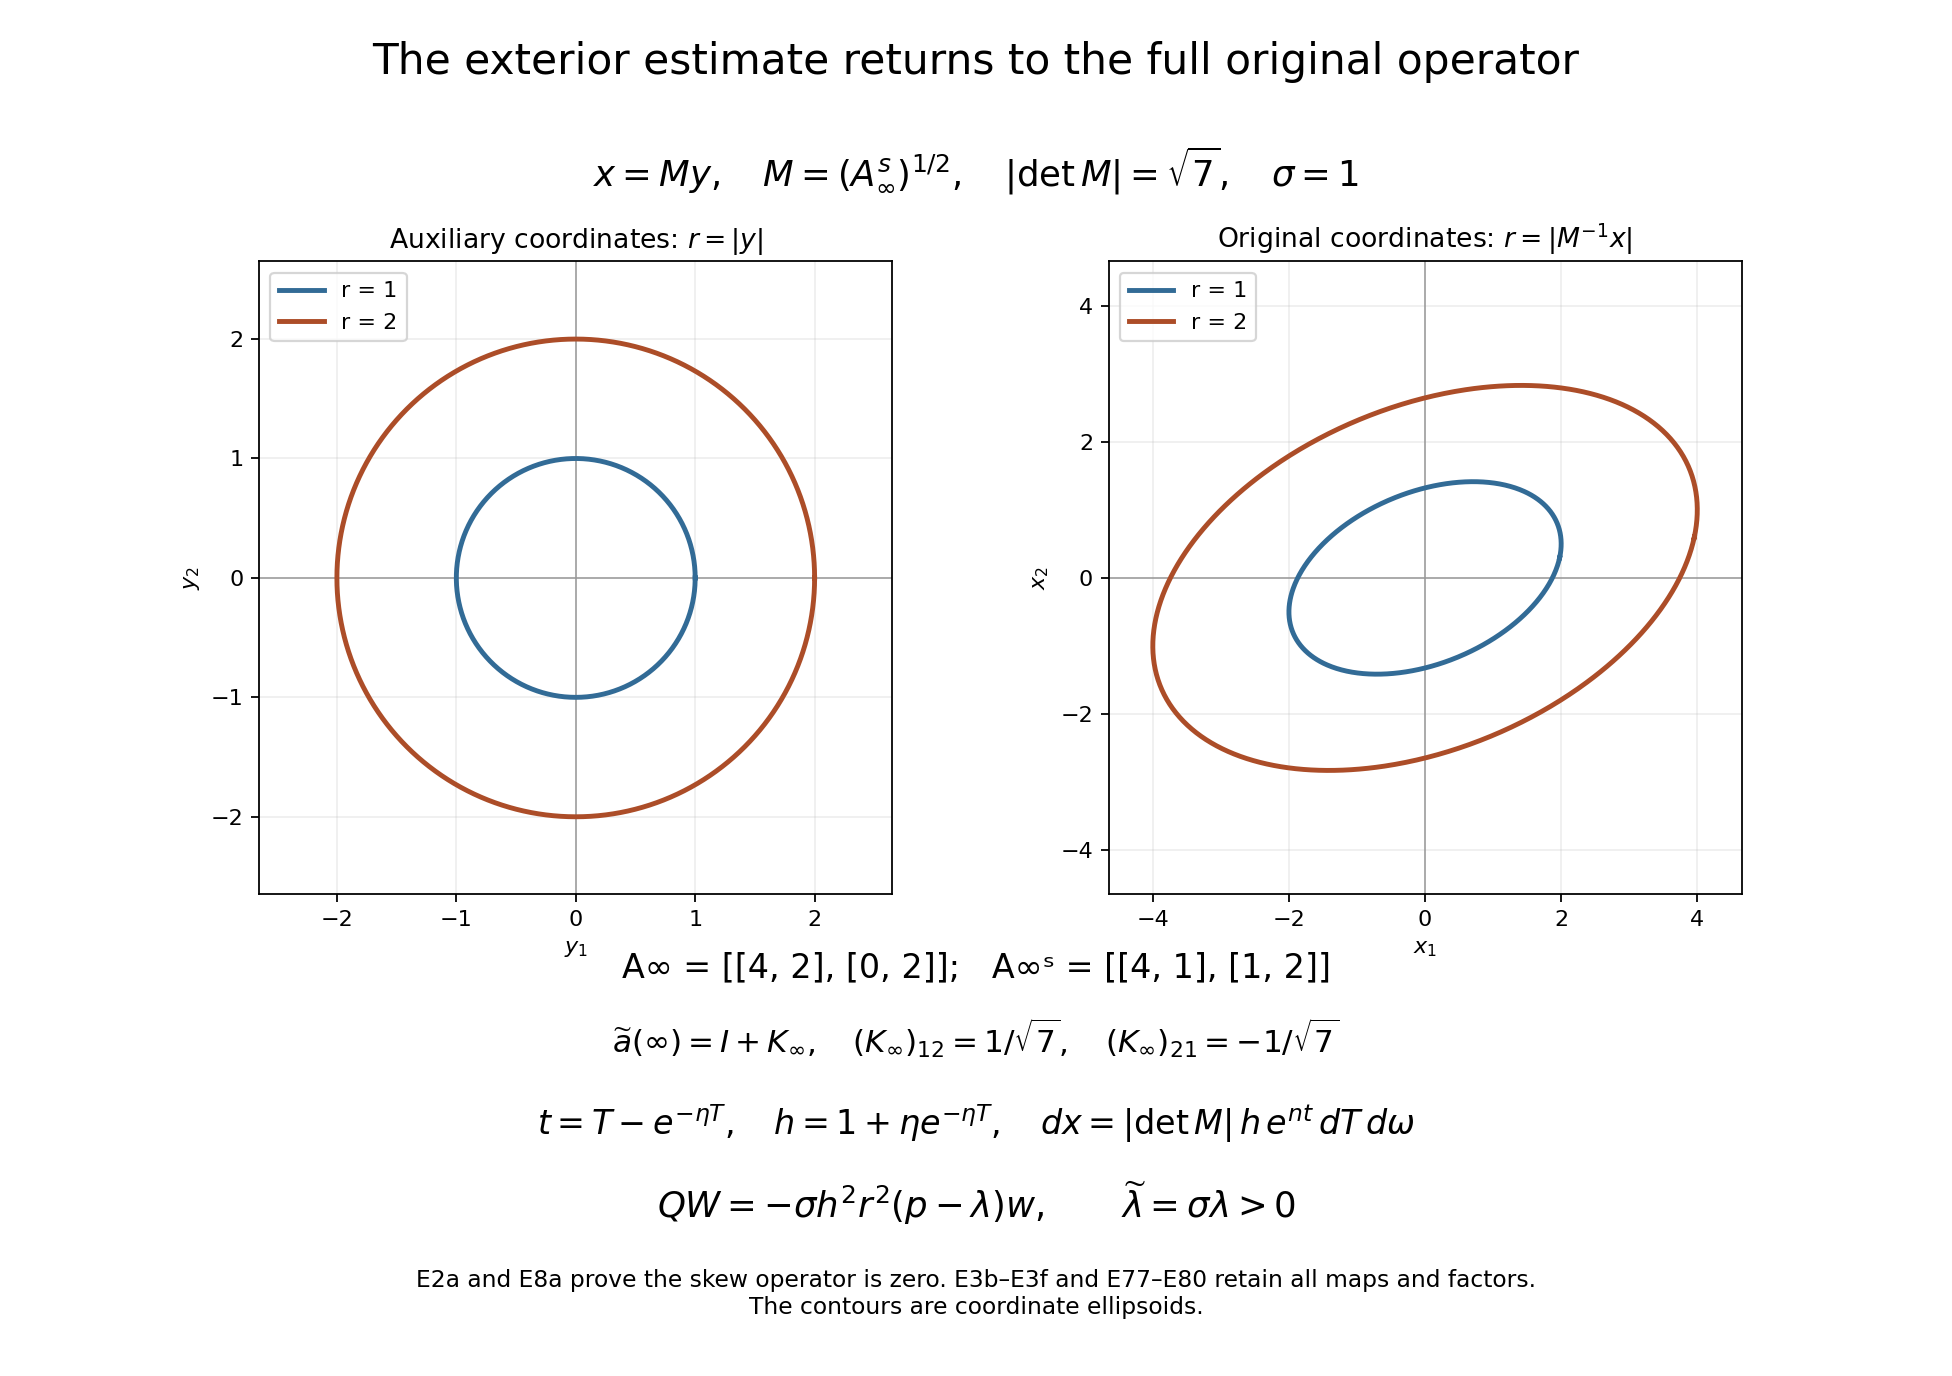
\includegraphics[keepaspectratio,alt={The full original exterior coordinates, matrix and measure}]{../figures/original-exterior-coordinate-map.png}}
\caption{The full original exterior coordinates, matrix and measure}
\end{figure}

For the displayed example,
\(A_\infty=\left(\begin{smallmatrix}4&2\\0&2\end{smallmatrix}\right)\),
\(\sigma=1\), and \(\det M=\sqrt7\). The full auxiliary matrix is
\(I+K_\infty\), with off-diagonal skew entries \(1/\sqrt7\) and
\(-1/\sqrt7\). The contours are the original coordinate surfaces
\(|M^{-1}x|=1,2\), rather than frequency surfaces. Equations
(E3b)--(E3f) and (E77)--(E80) prove every map and factor in the diagram.
This original-coordinate calculation makes no novelty claim.

\ReaderArmAliases{\ReaderOriginalAnchorStart{AN03-EXU-012}\ReaderOriginalAnchorEnd\begingroup\expandafter\def\csname @currentHref\endcsname{AN03-EXU-012}\label{AN03-EXU-012}\endgroup\ReaderOriginalAnchorStart{an03-exu-012-from-weak-decay-to-an-actual-open-zero-set}\ReaderOriginalAnchorEnd\begingroup\expandafter\def\csname @currentHref\endcsname{an03-exu-012-from-weak-decay-to-an-actual-open-zero-set}\label{an03-exu-012-from-weak-decay-to-an-actual-open-zero-set}\endgroup\ReaderOriginalAnchorStart{12-from-weak-decay-to-an-actual-open-zero-set}\ReaderOriginalAnchorEnd\begingroup\expandafter\def\csname @currentHref\endcsname{12-from-weak-decay-to-an-actual-open-zero-set}\label{12-from-weak-decay-to-an-actual-open-zero-set}\endgroup\ReaderOriginalAnchorStart{from-weak-decay-to-an-actual-open-zero-set}\ReaderOriginalAnchorEnd}
\subsection{12. From weak decay to an actual open zero
set}\label{from-weak-decay-to-an-actual-open-zero-set}

We prove the theorem of Section 1, beginning with the regularity needed
to use (E64).

On every compact subset of \(X\setminus\{0\}\), (E5) and
\(u\in H^1_{\mathrm{loc}}\) give \(pu\in L^2\). Weak elliptic regularity
in Sections 7--8 of \href{local-elliptic-coefficients.pdf}{Local inverses
and distance-weighted elliptic estimates} therefore gives
\(u\in H^2_{\mathrm{loc}}(X\setminus\{0\})\). The initially weak product
is \[
 aD_jv=D_j(av)-(D_ja)v,\qquad v\in L^2_{\mathrm{loc}}.
\] It agrees with the usual nondivergence expression after this
regularity improvement. In particular no second derivatives were assumed
in (E4).

We need this improvement with weights at infinity. Let
\(A_R=\{R<|x|<2R\}\) and \(A_R'=\{R/2<|x|<4R\}\). For sufficiently large
\(R\), both lie in \(X\). Scale \(x=Ry\) and write \(u_R(y)=u(Ry)\). The
coefficients \(a(Ry)\) on the fixed annulus \(\{1/2<|y|<4\}\) have
uniform ellipticity and a common modulus of continuity. Indeed they
approach the identity uniformly, and their first \(y\)-derivatives are
bounded by \(CR^{-1-d}\). The interior estimate in Section 6 of
\href{local-elliptic-coefficients.pdf}{Local inverses and
distance-weighted elliptic estimates}, on a fixed pair of nested annuli,
has a constant independent of \(R\). Scaling its \(m=p=2\) version back
yields \[
 \sum_{k=0}^2R^k\|D^ku\|_{L^2(A_R)}
       \leq C\left(R^2\|pu\|_{L^2(A_R')}
                                  +\|u\|_{L^2(A_R')}\right).    \tag{E65}
\] The same statement with a harmless separate first-order term on the
right would also suffice; it follows from the stated estimate by the
interior interpolation inequality. The factor \(R^{-n/2}\) from scaling
the \(L^2\) norm occurs on both sides and cancels.

By (E5), \[
 R^2\|pu\|_{L^2(A_R')}
       \leq C\left((R^2+R)\|u\|_{L^2(A_R')}
                                     +R\|Du\|_{L^2(A_R')}\right).
                                                                    \tag{E66}
\] For every \(N>0\), (E4) bounds the right side of (E66), and hence
every term on the left of (E65), by \(C_NR^{-N}\). To see this directly,
on \(A_R'\) the function \((1+|x|)^s\) is comparable to \(R^s\); take
\(s>N+2\) in (E4). It follows by summing dyadic annuli, whose enlarged
annuli have bounded overlap, that \[
 (1+|x|)^sD^\alpha u\in L^2(\{|x|>R_1\})
       \quad(s\in\mathbb R,\ |\alpha|\leq2).                    \tag{E67}
\] For a given \(s\), choose the annular exponent \(N\) larger than
\(s+1\); the squared annular estimates then sum as a convergent
geometric series.

Every cylindrical derivative through order two is a bounded sum of
\(e^{kt}D^ku(e^t\omega)\), \(k\leq2\). This follows by reversing (E7)
for first derivatives and then applying it again; derivatives of the
sphere factors are bounded. Using (E15), \(t-T\) bounded, and (E67), we
conclude \[
 e^{qT}\mathcal D^kU\in L^2((T_1,\infty)\times S^{n-1})
                     \quad(q\in\mathbb R,\ 0\leq k\leq2).       \tag{E68}
\] For instance, the measure conversion for the \(k\)-th Cartesian
contribution changes a squared exponential weight \(e^{2qT}\) into a
fixed radial power comparable to \(r^{2q+2k-n}\); (E67) allows every
such power. This checks the Jacobian, rather than inferring (E68) from a
pointwise assertion of decay.

Fix \(T_0\) above the thresholds used in the Carleman estimate. Choose a
real smooth cutoff \(\chi\), zero for \(T\leq T_0+1\) and one for
\(T\geq T_0+2\). Let \(\theta_L\) be one for \(T\leq L\), zero for
\(T\geq L+1\), with first two derivatives bounded independently of
\(L\). Apply (E64), by its \(H^2\) extension, to \[
                            U_L=\chi\theta_LU.                  \tag{E69}
\] For a fixed \(\tau\), (E68) permits \(L\to\infty\) in every term. In
detail, all upper-cutoff commutators are supported in \([L,L+1]\) and
are bounded by \(C(|U|+|\mathcal D^1U|)\), since the potential commutes
and \(Q\) has bounded differential coefficients. Their weighted \(L^2\)
norms tend to zero by (E68). Equation (E14) makes \(e^{\tau T}QU\)
square integrable, so the noncommutator terms converge as well.
Derivatives on the left converge by the same argument. Thus (E64) holds
for \(\chi U\). Smoothing occurs first for each compactly supported
\(U_L\), then \(L\to\infty\) at fixed \(\tau\), and only later will
\(\tau\to\infty\).

Write \[
 S_\tau(W)=\|e^{(\tau+1)T}W\|^2
            +\|e^{\tau T}\mathcal D^1W\|^2,\qquad
                      m_0=e^{-T_0/2}+\tau^{-1}.
\] Using (E14), the product rule, and
\(\chi\mathcal D U=\mathcal D(\chi U)-(\mathcal D\chi)U\), we obtain \[
 \|e^{\tau T}Q(\chi U)\|^2
           \leq C_1 S_\tau(\chi U)+C_2e^{2\tau(T_0+2)}H_0^2.   \tag{E70}
\] Here \(H_0\) is a fixed finite norm of \(U,\mathcal D^1U\) on the
transition strip \([T_0+1,T_0+2]\), with any fixed bounded weight such
as \(e^T\) included. It is independent of \(\tau\). The constants
controlling the equation near infinity are uniform in the strip position
once the initial threshold is fixed.

By (E64) and (E70), \[
 S_\tau(\chi U)\leq C m_0 C_1 S_\tau(\chi U)
                      +C m_0 C_2e^{2\tau(T_0+2)}H_0^2.
\] Increase the fixed \(T_0\), then the lower threshold for \(\tau\),
until \(CC_1m_0\leq1/2\). Absorb the first right-side term. For each
fixed \(\sigma>0\), restrict the zeroth-order norm to
\(T>T_0+2+\sigma\), where \(\chi=1\), to deduce \[
 \|e^TU\|_{L^2(T>T_0+2+\sigma)}^2
                   \leq C m_0e^{-2\tau\sigma}H_0^2.             \tag{E71}
\] Let \(\tau\to\infty\). The right side tends to zero with
\(T_0,\sigma\) fixed. Taking a countable union of these regions as
\(\sigma\downarrow0\) proves \(U=0\) for \(T>T_0+2\). We have obtained a
nonempty exterior open zero set for \(u\).

It remains to justify continuation throughout \(X\). In dimensions
greater than two, Section 8 of \href{support-continuation.pdf}{Curved
weights and the directions in which support can end} says that every
real normal is admissible for every elliptic complex quadratic form. In
dimension two, choose independent real covectors \(\xi,N\). The two
roots of \[
                       z\longmapsto p_x(\xi+zN)                 \tag{E72}
\] cannot cross the real axis as \(x\) varies, by ellipticity, and their
upper-half-plane count is locally constant. Far out,
\(\operatorname{Re}p_x\) is positive definite. The path
\(\operatorname{Re}p_x+i s\operatorname{Im}p_x\), \(0\leq s\leq1\),
stays elliptic. At \(s=0\) its roots are a nonreal conjugate pair, so
the upper count is one also at \(s=1\). Connectedness of \(X\) makes the
same count equal to one everywhere. Thus a double nonreal root never
occurs, and every real normal is admissible throughout \(X\). This
argument uses asymptotic positivity; it does not assert that
\(a_{jk}(x)\) are real at some finite point.

On \(X\setminus\{0\}\), the local equation has bounded lower-order
coefficients on compact sets. Section 7 of
\href{support-continuation.pdf}{Curved weights and the directions in
which support can end} therefore excludes every normal to a proper
support boundary. Its open-set propagation consequence gives \(u=0\) on
this domain. When \(n\geq2\), removing one point from a connected open
set leaves it connected: a polygonal path can be modified inside a
sufficiently small ball about the removed point by an arc on a sphere,
without leaving the open set. If \(0\in X\), its singleton is a null
set, so vanishing off zero proves the asserted almost-everywhere
conclusion on \(X\).

For \(n=1\), a connected open neighborhood of both ends of the line is
the whole line. Interpret \(S^0\) as its two points, with counting
measure; the angular fields and their sums are zero. The polar identity
is \(\partial_t^2-\partial_t\), which is (E9) for \(n=1\). All estimates
above remain valid on the two half-cylinders. The Fourier shell in
Section 4 is empty in this case; its off-shell estimate suffices. The
proof of (E52) used only boundedness of \(c\) and \(c'\), so also
applies. The two exterior tails vanish. In dimension one a nonzero
quadratic symbol has no exceptional nonzero normal, by Section 8 of
\href{support-continuation.pdf}{Curved weights and the directions in
which support can end}. Propagate from the two tails on the two
components of \(X\setminus\{0\}\), and ignore the null singleton. The
same reasoning proves a one-ended version on a half-line which avoids
the origin; if a half-line crosses zero, propagation across it needs a
locally bounded differential inequality there. The singular inequality
(E5) alone does not supply that additional conclusion. This completes
the theorem in every dimension. \(\square\)

\ReaderArmAliases{\ReaderOriginalAnchorStart{AN03-EXU-TAIL-001}\ReaderOriginalAnchorEnd\begingroup\expandafter\def\csname @currentHref\endcsname{AN03-EXU-TAIL-001}\label{AN03-EXU-TAIL-001}\endgroup\ReaderOriginalAnchorStart{polynomial-weights-on-one-tail-suffice-for-the-solution-alone}\ReaderOriginalAnchorEnd}
\subsubsection{12.1. Polynomial weights on one tail suffice for the
solution
alone}\label{polynomial-weights-on-one-tail-suffice-for-the-solution-alone}

The proof of Section 12 uses weighted norms only on an exterior region.
Its first-derivative assumption follows from an energy estimate there.
We prove that implication without assuming global integrability near a
finite boundary of the original domain.

\textbf{Corollary.} Retain (E1)--(E3), \(\lambda>0\),
\(u\in H^1_{\mathrm{loc}}(X)\), the inequality (E5) near infinity, and
the locally bounded continuation inequality on compact subsets of
\(X\setminus\{0\}\). In place of (E4), it suffices to assume, for one
exterior radius \(R_u\), \[
 (1+|x|)^s u\in L^2(\{|x|>R_u\})
 \quad\text{for every real }s.
 \tag{ECT1}
\] Then the original solution vanishes almost everywhere on \(X\). The
two-ended dimension-one formulation and the qualification for a
half-line crossing zero remain exactly those in Section 12. For the full
real definite limiting matrix (E3a), the same conclusion holds with the
original required energy sign \(\sigma\lambda>0\). No all-weight
derivative assumption, or global integrability approaching a finite
boundary of \(X\), is required.

\textbf{Coercivity of the full complex matrix on a large annulus.}
Select \(R_0\geq1\) so large that, for every \(R\geq R_0\), the closure
of \[
 A_R'=\{R/2<|x|<4R\}
\] lies inside the region where (E3) and (E5) hold and inside \(X\).
Increase \(R_0\) to ensure \(nC_a(R_0/2)^{-1-\delta}\leq1/2\). The
entrywise bound gives
\(\|A-I\|_{\mathrm{op}}\leq n\max_{j,k}|a_{jk}-\delta_{jk}|\leq1/2\).
Indeed for a complex vector \(z\), each component of \((A-I)z\) has
absolute value at most the entry maximum times
\(\sum_k|z_k|\leq\sqrt n|z|\); summing its \(n\) component squares
proves the displayed norm bound. Consequently \[
 \operatorname{Re}\sum_{j,k}a_{jk}z_k\overline{z_j}
 \geq\tfrac12|z|^2,\qquad \|A\|_{\mathrm{op}}\leq\tfrac32
 \quad(x\in A_R',\ z\in\mathbb C^n).
 \tag{ECT2}
\] This uses the full complex sesquilinear expression. Positivity on
complex vectors has not been inferred merely from the real-covector
ellipticity assumption.

\textbf{The full annular energy identity.} Choose a real smooth cutoff
\(\chi_0\), with \(0\leq\chi_0\leq1\), equal to one on
\(1\leq|y|\leq2\), compactly supported in \(1/2<|y|<4\), and put
\(C_\chi=\|\nabla\chi_0\|_\infty\). Set \(\chi_R(x)=\chi_0(x/R)\),
\(A_R=\{R<|x|<2R\}\), and retain \[
 \begin{gathered}
 q=(p_A-\lambda)u,\qquad b_k=\sum_j\partial_j a_{jk},\\
 b_R=n^{3/2}C_a(R/2)^{-2-\delta},\qquad
 |b(x)|\leq b_R,\quad
 |q(x)|\leq(2C/R)(|u(x)|+|\nabla u(x)|),\\
 U=\|u\|_{L^2(A_R')},\quad
 G=\|\chi_R\nabla u\|_2,\quad
 H=\|u\nabla\chi_R\|_2\leq C_\chi U/R.
 \end{gathered}                                                   \tag{ECT3}
\] The coefficient \(n^{3/2}\) follows by bounding each of the \(n\)
terms in each \(b_k\) by \(C_a(R/2)^{-2-\delta}\), and then taking the
Euclidean norm of its \(n\) components. On the cutoff support, the
original inequality and local \(H^1\) regularity give \(p_Au\in L^2\).
Sections 7--8 of \href{local-elliptic-coefficients.pdf}{Local inverses
and distance-weighted elliptic estimates} give \(H^2\) on a neighborhood
of that support. The weak integration identity can therefore be proved
by \(H^2\) approximation and the Lipschitz product rule. Its exact
nondivergence form is \[
 \begin{split}
 \int(p_Au)\chi_R^2\bar u
 ={}&\sum_{j,k}\int a_{jk}\partial_k u
       \bigl(\chi_R^2\partial_j\bar u
              +2\chi_R(\partial_j\chi_R)\bar u\bigr)\\
 &+\sum_k\int b_k\partial_k u\,\chi_R^2\bar u.
 \end{split}                                                     \tag{ECT4}
\] All integrals are over the cutoff support, extended by zero outside
it. The plus signs result from \(p_A=-\sum a_{jk}\partial_j\partial_k\),
with one integration by parts in \(x_j\). The original full skew
entries, their derivative contribution to \(b\), and both cutoff terms
remain in this identity.

Take real parts and use \(p_Au=\lambda u+q\), (ECT2), Cauchy--Schwarz,
and \(0\leq\chi_R\leq1\). The equation term is bounded by
\((\lambda+2C/R)U^2+(2C/R)GU\). The coefficient derivative term is
bounded by \(b_RGU\). The cutoff cross term is bounded by
\(2\|A\|_{\mathrm{op}}GH\leq3GH\). Thus \[
 \tfrac12G^2\leq(\lambda+2C/R)U^2+L_RGU,
 \qquad L_R=(2C+3C_\chi)/R+b_R.
 \tag{ECT5}
\] The exact inequality \(L_RGU\leq G^2/4+L_R^2U^2\) follows by squaring
\(G/2-L_RU\). Since \(\chi_R=1\) on \(A_R\), it yields \[
 \|\nabla u\|_{L^2(A_R)}^2\leq G^2
 \leq4\bigl(\lambda+2C/R+L_R^2\bigr)
                    \|u\|_{L^2(A_R')}^2.
 \tag{ECT6}
\] Every term of \(L_R\) decreases for \(R\geq R_0\). We therefore have
the explicit common finite bound \[
 C_{\mathrm{ext}}=4\bigl(\lambda+2C/R_0+L_{R_0}^2\bigr)
 \tag{ECT7}
\] for the entire right coefficient. No weighted derivative assumption
entered the proof.

\textbf{Every weighted gradient tail follows.} For \(s\in\mathbb R\),
the ratio of the maximum of \((1+r)^{2s}\) on \(R<r<2R\) to its minimum
on \(R/2<r<4R\) is at most \(6^{2|s|}\). For \(s\geq0\), use
\((1+2R)/(1+R/2)\leq4\); for \(s<0\), use \((1+4R)/(1+R)\leq4\). Both
are in particular at most six, and the sign of \(s\) determines which
endpoint is the maximum. Multiplying (ECT6) by that maximum gives the
full comparison \[
 \int_{A_R}(1+|x|)^{2s}|\nabla u|^2dx
 \leq C_{\mathrm{ext}}6^{2|s|}
              \int_{A_R'}(1+|x|)^{2s}|u|^2dx.
 \tag{ECT8}
\] Use \(R=2^kR_0\), \(k\geq0\). The annuli \(A_R\) cover \(|x|>R_0\) up
to their sphere boundaries, which have Lebesgue measure zero. For a
given positive radius, membership in an enlarged annulus requires
\(k-1<\log_2(r/R_0)<k+2\); at most four integer indices meet this
condition. All these enlarged annuli lie in \(|x|>R_0/2\). Summing
nonnegative integrals therefore proves \[
 \int_{|x|>R_0}(1+|x|)^{2s}|\nabla u|^2dx
 \leq4C_{\mathrm{ext}}6^{2|s|}
             \int_{|x|>R_0/2}(1+|x|)^{2s}|u|^2dx<\infty.
 \tag{ECT9}
\] The right integral is finite by (ECT1) outside the larger of \(R_u\)
and \(R_0/2\). The intervening closed bounded annulus is compactly
contained in \(X\), and its weight is bounded, so local \(H^1\) supplies
its finite integral. This is a local argument on a compact subset, not
an assumption of integrability near an arbitrary finite boundary of
\(X\).

Now (E65)--(E66) use only the original solution and first-derivative
norms on those enlarged exterior annuli. They give every
second-derivative tail weight (E67), and the full radial Jacobian gives
every cylinder weight (E68). The entire cutoff argument (E69)--(E71)
consequently applies, with its original order of limits, to obtain the
same exterior open zero set. The root-count and compact-set continuation
argument (E72), including its dimension-one qualifications, then gives
\(u=0\) almost everywhere on the original \(X\). This proves the
corollary without invoking the preceding theorem under an unmet global
version of (E4). \(\square\)

\textbf{Returning a full definite limiting matrix.} Keep every datum in
(E3a)--(E3f). The exact auxiliary field is
\(\widetilde A=\sigma M^{-1}A(My)M^{-T}\), with limit \(I+K_\infty\),
rather than \(I\). Introduce its symmetric part
\(\widetilde B=(\widetilde A+\widetilde A^T)/2\) for the energy
estimate. Formulas (E2a) and (E8a), with the same weak product argument
as (ECT4), prove \(p_{\widetilde B}=p_{\widetilde A}\) on punctured
compact sets. Its limit is exactly \(I\). The full entry and derivative
comparisons in (E3d) give its two required decay bounds, since averaging
a pair of entries retains those bounds with their displayed matrix sums.
Apply (ECT2)--(ECT9) to this auxiliary symmetric field and positive
energy \(\widetilde\lambda=\sigma\lambda\), retaining the exact
inequality (E3e).

The original solution tail (ECT1) transfers to \(v=u\circ M\) by the
actual singular-value inequalities in (E3f). Choose the auxiliary
threshold large enough that \(m_-R_0/2\) exceeds every original
coefficient, equation and domain threshold. For each exterior radius
\(R\), the exact restricted measure and gradient identity is \[
 \begin{split}
 &\int_{|y|>R}(1+|My|)^{2s}
             \bigl(|v|^2+|M^{-T}D_yv|^2\bigr)\,dy\\
 &\qquad=|\det M|^{-1}
      \int_{|M^{-1}x|>R}(1+|x|)^{2s}
             \bigl(|u|^2+|D_xu|^2\bigr)\,dx.
 \end{split}                                                     \tag{ECT10}
\] The inverse gradient entries and both singular-value weight constants
in (E3f) show its finiteness after (ECT9). The region \(|x|>m_+R\) is
contained in \(|M^{-1}x|>R\), so it supplies an actual original radial
gradient tail as well. Sections 2--12 then return the exterior zero set
through the complete maps (E77)--(E80). All original skew data, the sign
\(\sigma\), energy \(\lambda\), gradient \(M^{-T}D_yv\), integration
regions and determinant remain explicit.

\textbf{Equivalent tests for the weight quantifier.} It is enough to
test (ECT1) on any real sequence \(s_l\) tending to \(+\infty\),
including the nonnegative integers. For a fixed real \(s\), select
\(s_l\geq s\). Since \(1+|x|\geq1\), the exact inequality
\((1+|x|)^{2s}\leq(1+|x|)^{2s_l}\) bounds the required squared integral
by that tested one. Conversely all real weights include every selected
sequence. This proves the equivalence for the original solution and,
after (ECT9), its derivative tail, without changing their measures or
domains.

\begin{figure}
\centering
\pandocbounded{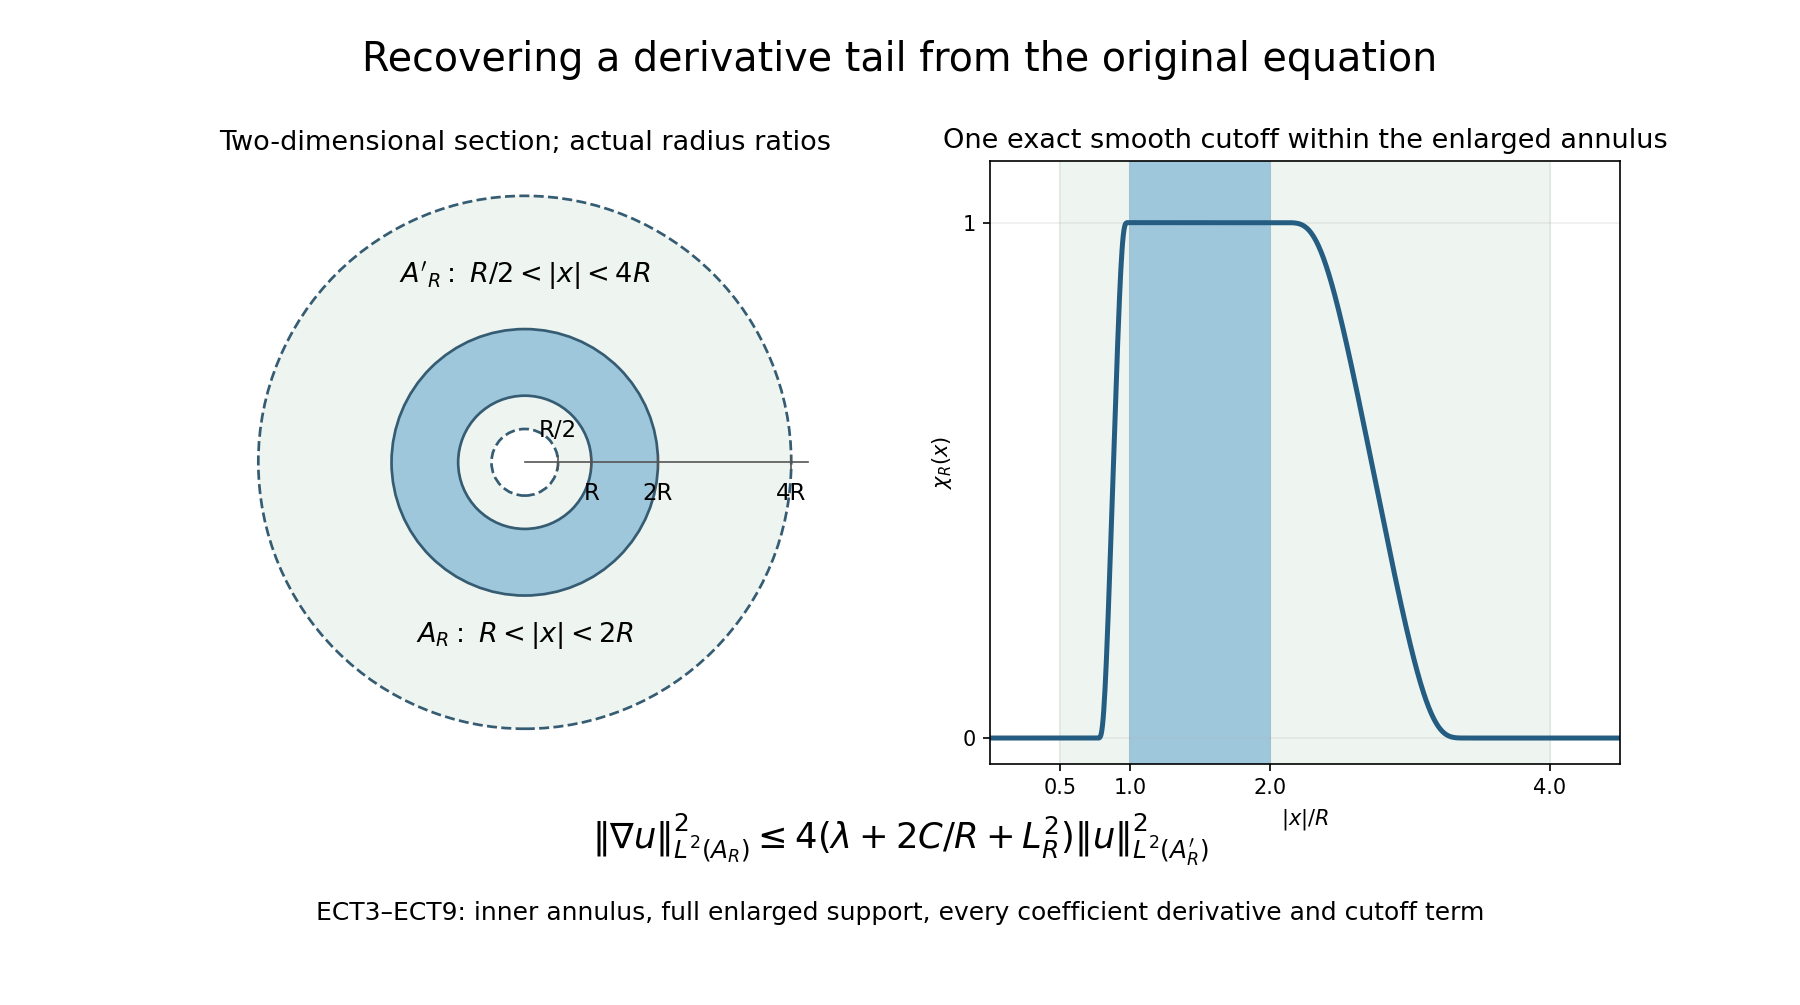
\includegraphics[keepaspectratio,alt={The exact inner and enlarged annuli used for the exterior energy estimate}]{../figures/continuation-caccioppoli-annuli.png}}
\caption{The exact inner and enlarged annuli used for the exterior
energy estimate}
\end{figure}

The drawing is a two-dimensional section of the \(n\)-dimensional
supports in (ECT3)--(ECT9), with all four radii in their actual ratio.
Its displayed cutoff is the exact function \[
 \begin{gathered}
 h(t)=\begin{cases}e^{-1/t},&t>0,\\0,&t\leq0,\end{cases}
 \qquad \eta(t)=\frac{h(t)}{h(t)+h(1-t)},\\
 \chi_0(y)=\eta(4|y|-3)\eta\bigl((7-2|y|)/3\bigr).
 \end{gathered}                                                   \tag{ECT11}
\] The denominator is everywhere positive. Repeated derivatives of \(h\)
on the positive ray are a finite polynomial in \(t^{-1}\) times
\(e^{-1/t}\); they all tend to zero at zero. Thus \(h\) and \(\eta\) are
smooth, with \(\eta=0\) on \(t\leq0\) and \(\eta=1\) on \(t\geq1\). This
\(\chi_0\) is zero for \(|y|\leq3/4\) and \(|y|\geq7/2\), equals one for
\(1\leq|y|\leq2\), and is smooth even at the origin because it vanishes
in a neighborhood there. Its support is compactly contained in the
enlarged annulus, and its smooth gradient has finite maximum \(C_\chi\).
This verifies every cutoff property used in (ECT3) for the actual
drawing.

This annular argument is a consequence of the complete exterior proof
here. Exact original-author source comparison for the stronger tail
formulation remains separate, and no historical novelty is claimed. The
original theorem and its solutions remain intact. In particular the
outgoing wave (E75) still fails the required all-weight condition on the
solution itself, and the negative-energy example (E74) still prevents
deletion of the energy sign.

\ReaderArmAliases{\ReaderOriginalAnchorStart{AN03-EXU-013}\ReaderOriginalAnchorEnd\begingroup\expandafter\def\csname @currentHref\endcsname{AN03-EXU-013}\label{AN03-EXU-013}\endgroup\ReaderOriginalAnchorStart{an03-exu-013-worked-models-and-precise-nonconclusions}\ReaderOriginalAnchorEnd\begingroup\expandafter\def\csname @currentHref\endcsname{an03-exu-013-worked-models-and-precise-nonconclusions}\label{an03-exu-013-worked-models-and-precise-nonconclusions}\endgroup\ReaderOriginalAnchorStart{13-worked-models-and-precise-nonconclusions}\ReaderOriginalAnchorEnd\begingroup\expandafter\def\csname @currentHref\endcsname{13-worked-models-and-precise-nonconclusions}\label{13-worked-models-and-precise-nonconclusions}\endgroup\ReaderOriginalAnchorStart{worked-models-and-precise-nonconclusions}\ReaderOriginalAnchorEnd}
\subsection{13. Worked models and precise
nonconclusions}\label{worked-models-and-precise-nonconclusions}

\textbf{A complex angular perturbation at the allowed regularity.} Let
\(B(\omega)\) be a real symmetric matrix with Lipschitz entries on the
sphere, and put, on \(r>2\), \[
               a(x)=I+i r^{-1-\delta}B(x/r).                    \tag{E73}
\] For real \(\xi\), \(\operatorname{Re}(\xi^ta\xi)=|\xi|^2\), so
ellipticity is immediate, independently of the size of \(B\). Radial
differentiation of \(r^{-1-\delta}\) gives \(O(r^{-2-\delta})\), and
angular differentiation of \(B(x/r)\) introduces one factor \(r^{-1}\).
Thus (E3) holds almost everywhere. If measurable lower-order
coefficients satisfy \[
 |\beta(x)|+|\gamma(x)|\leq C/r,
\] then every solution of \[
                  (p+\beta\cdot D+\gamma-\lambda)u=0
\] at the stated weak \(H^1\) regularity satisfies (E5). For
\(\lambda>0\), (E4) forces that solution to vanish. This example allows
genuinely complex leading coefficients and merely Lipschitz angular
dependence. It does not use a self-adjoint realization of the operator.

\textbf{The sign of the energy changes the answer.} In dimension three,
set \[
               u(x)=\frac{e^{-\kappa|x|}}{|x|},
               \qquad |x|>2,\quad \kappa>0.                    \tag{E74}
\] For a radial function \(f(r)\), \(\Delta f=f''+2f'/r\). Here \[
 f'=-e^{-\kappa r}(\kappa/r+1/r^2),\qquad
 f''=e^{-\kappa r}(\kappa^2/r+2\kappa/r^2+2/r^3),
\] so \(\Delta u=\kappa^2u\). Therefore \((-\Delta-\lambda)u=0\) with
\(\lambda=-\kappa^2\), and \(u,Du\) belong to every polynomially
weighted \(L^2\) space on the exterior. The function is nonzero.
Equivalently, for the negative-definite symbol of \(p=\Delta\), the same
function solves \((p-\kappa^2)u=0\) at positive energy. Thus the
relative sign cannot be discarded when comparing a general real elliptic
limiting quadratic form with its auxiliary expression.

\textbf{A polynomially weighted solution which does not satisfy all
weights.} Still in dimension three, let \[
                    u(x)=\frac{e^{ik|x|}}{|x|},
                    \qquad |x|>2,\quad k>0.                    \tag{E75}
\] The same radial calculation, with \(\kappa=-ik\), gives
\((-\Delta-k^2)u=0\). Since \(|u|=r^{-1}\) and
\(|u'|^2=k^2r^{-2}+r^{-4}\), both weighted integrals for \(u\) and
\(Du\) behave at infinity like \(\int_2^\infty r^{2s}\,dr\). They are
finite exactly when \(s<-1/2\). This provides many weighted \(L^2\)
conditions, but not (E4); there is no contradiction with the theorem.

\textbf{Small values do not control coefficient derivatives.} Consider
\[
               a(x)=\bigl(1+i r^{-1-\delta}\sin(r^3)\bigr)I
                 \quad(r>2).                                  \tag{E76}
\] Its real part is the identity and its distance from \(I\) satisfies
the first bound in (E3). Its radial derivative contains
\(3i r^{1-\delta}\cos(r^3)\), so the second bound in (E3) fails. The
theorem has not been proved under only the first bound. This example
identifies a missing assumption in an attempted application; it is not a
counterexample to a more general uniqueness theorem.

These examples isolate four different issues: complex coefficients, the
sign of the limiting form relative to the energy, quantification over
all weights, and independent control of first coefficient derivatives.

\ReaderArmAliases{\ReaderOriginalAnchorStart{AN03-EXU-014}\ReaderOriginalAnchorEnd\begingroup\expandafter\def\csname @currentHref\endcsname{AN03-EXU-014}\label{AN03-EXU-014}\endgroup\ReaderOriginalAnchorStart{an03-exu-014-problems-with-complete-solutions}\ReaderOriginalAnchorEnd\begingroup\expandafter\def\csname @currentHref\endcsname{an03-exu-014-problems-with-complete-solutions}\label{an03-exu-014-problems-with-complete-solutions}\endgroup\ReaderOriginalAnchorStart{14-problems-with-complete-solutions}\ReaderOriginalAnchorEnd\begingroup\expandafter\def\csname @currentHref\endcsname{14-problems-with-complete-solutions}\label{14-problems-with-complete-solutions}\endgroup\ReaderOriginalAnchorStart{problems-with-complete-solutions}\ReaderOriginalAnchorEnd}
\subsection{14. Problems with complete
solutions}\label{problems-with-complete-solutions}

\textbf{Problem 1: anisotropy and the unchanged decay exponents.} In
\(\mathbb R^3\), suppose the coefficient matrix tends to
\(G=\operatorname{diag}(4,1,9)\) with the two rates in (E3). Find the
full linear coordinate comparison, retain the original matrix and
Jacobian, and determine the energy sign required by the theorem.

\textbf{Solution.} Put \(x=(2y_1,y_2,3y_3)\), so
\(S=G^{1/2}=\operatorname{diag}(2,1,3)\). The chain rule gives
\(D_x=S^{-t}D_y\); hence the new coefficient matrix is \[
              \widetilde a(y)=S^{-1}a(Sy)S^{-t}.
\] Its limit is \(S^{-1}GS^{-t}=I\). Since \(|y|\leq|Sy|\leq3|y|\), the
error is \(O(|y|^{-1-\delta})\). Differentiating \(a(Sy)\) introduces
only a fixed matrix factor, giving \(O(|y|^{-2-\delta})\). The Jacobian
is the constant \(\det S=6\). Formula (E3f), with \(m_-=1,m_+=3\), gives
the exact weighted integral and both comparisons for every real
exponent. Formula (E79) retains that factor six, every radial and \(h\)
factor, and the original \(p-\lambda\) in its original coordinates;
(E80) supplies every original derivative. The spectral parameter is
unchanged because the change of variables has not multiplied the
equation by a scalar. Thus the required sign is \(\lambda>0\). If the
limit were \(-G\), multiplication by \(-1\) would replace the energy by
\(-\lambda\); the theorem would require the original \(\lambda<0\).

\textbf{Problem 2: locate the three regimes without losing a parameter.}
Take \(A\geq1\), \(\eta=1/2\), and \(\tau=A^q\) with \(q>0\). Compute
the choice (E31), identify both transition exponents, and check
\(K\geq A\).

\textbf{Solution.} For \(A>1\), the conditions \(\tau^2\leq A^2\) and
\(\tau^2\geq A^{2+\eta}\) become \(q\leq1\) and \(q\geq5/4\). When
\(A=1\), one has \(\tau=K=1\), and all the expressions agree for every
\(q\). For \(A>1\) the regimes give \[
 K=
 \begin{cases}
 A^{2-q},&0<q\leq1,\\
 A^{3q-2},&1\leq q\leq5/4,\\
 A^{q+1/2},&q\geq5/4.
 \end{cases}
\] At \(q=1\), the first two exponents are both one. At \(q=5/4\), the
last two exponents are both \(7/4\). Every exponent is at least one in
its designated range, proving \(K\geq A\). Moreover \(\tau A^2/K\)
equals \(A^{2q}\), \(A^{4-2q}\), and \(A^{3/2}\), respectively. The
middle exponent is at least \(3/2\), which checks the condition
\(M^2K\leq\tau A^2\) when \(M\leq\min(A^{3/4},\tau)\).

\textbf{Problem 3: why the second-derivative error has its stated
weight.} Bound \[
 I_j=\int e^{-(1+d)T}\tau^j|\mathcal D^2V|\,|\mathcal D^sV|,
          \qquad j+s\leq1,
\] by \(R(V)\). Explain why replacing its first term by an unweighted
\(H^1\) norm does not follow from the same argument.

\textbf{Solution.} Factor the integrand as in (E20) and apply
\(2ab\leq a^2+b^2\): \[
 I_j\leq\tfrac12\tau^{-1}\|e^{-T}\mathcal D^2V\|^2
       +\tfrac12\tau^{2j+1}\|e^{-dT}\mathcal D^sV\|^2.
\] Since \(2j+1\leq3-2s\), the second term is at most half the
corresponding term in \(R\). The first term is exactly its order-two
term. There is no pointwise or unrestricted norm inequality bounding two
derivatives by one derivative. For example a fixed compactly supported
amplitude multiplied by \(e^{iky_1}\) in a chart has second-derivative
norm growing like \(k^2\), while its first-derivative norm grows like
\(k\). The separate Fourier estimate, involving \(Q_\tau V\), is what
eventually controls that order-two contribution.

\textbf{Problem 4: a lower limit for the shell parameter.} Assume (E24)
and (E30). Prove the necessary lower bound (E35), and explain why
\(\tau^3/A^2\) cannot be used for \(K\) in all three regions.

\textbf{Solution.} Rearranging the second inequality of (E24) gives
\(K\geq\tau^3/(A^{-\eta}\tau^2+A^2)\); (E30) gives \(K\geq A^2/\tau\).
Their maximum is (E35). If \(K=\tau^3/A^2\) and \(\tau<A\), then
\(A^2/K=A^4/\tau^3>\tau\), violating (E30). If \(\tau^2>2A^{2+\eta}\),
then \(A^{-\eta}\tau^2>2A^2=\tau^3/K+A^2\), violating the first
inequality in (E24). Thus the middle expression fails in both
sufficiently extreme regions, for two different reasons.

\textbf{Problem 5: the endpoint cutoff limit and its order.} Suppose
only (E68) and (E14) are known, and \(\chi,\theta_L\) are as in (E69).
Show that the upper-cutoff error disappears for each fixed \(\tau\), and
explain why this is not a uniform statement as \(\tau\to\infty\).

\textbf{Solution.} Every derivative of \(\theta_L\) is supported in
\([L,L+1]\), with a bound independent of \(L\). Since the coefficients
of the differential part of \(Q\) are bounded, the product rule gives \[
 \|e^{\tau T}[Q,\theta_L](\chi U)\|
    \leq C\|e^{\tau T}(|U|+|\mathcal D^1U|)\|_{L^2(L<T<L+1)}
\] for \(L>T_0+3\). The right side tends to zero as a tail of a fixed
\(L^2\) function, by (E68). The potential contributes no commutator.
Also \(e^{\tau T}QU\in L^2\) by (E14) and the \(q=\tau+1,\tau\) cases of
(E68), so multiplication by \(\theta_L\) converges on the equation term.
Nothing in (E68) bounds the norms uniformly over all \(q\); the
constants may grow arbitrarily with \(q\). Therefore the justified order
is smoothing on a fixed compact set, removing the upper cutoff at fixed
\(\tau\), and then sending \(\tau\) to infinity in the already
established estimate.

\textbf{Problem 6: propagation without a real coefficient point.}
Suppose \(n=2\), \(X\) is connected, the quadratic principal forms are
continuous and elliptic, and their real parts are positive definite at
one point. Prove that every line polynomial (E72), with independent real
\(\xi,N\), has one root in each open half-plane throughout \(X\).
Explain the consequence for a locally Lipschitz equation which vanishes
on an exterior open set.

\textbf{Solution.} At the selected point, the path that multiplies the
imaginary part of the form by \(s\in[0,1]\) keeps its positive real part
and hence remains elliptic. At \(s=0\), the real quadratic polynomial in
the line parameter has no real roots and therefore has a conjugate pair.
The upper-half-plane count is one. A root cannot cross the real axis
along this path, so the same count holds for the original complex form
at that point. For a fixed independent pair \(\xi,N\), continuity of the
unordered two-root set, including multiplicities, follows from the
quadratic formula. Ellipticity prevents real roots everywhere in \(X\),
and the leading coefficient \(p_x(N)\) never vanishes. Consequently the
upper count is locally constant and hence constant on connected \(X\).
It remains one. The roots are distinct, since a double root would put
both in one half-plane. The same argument applies to every independent
pair; dependent pairs only give the zero complex vector excluded from
the exceptional-normal definition. Thus the exceptional normal set is
empty. Section 7 of \href{support-continuation.pdf}{Curved weights and
the directions in which support can end} then propagates any nonempty
open zero set through a connected region where the lower-order
inequality has locally bounded coefficients. The proof used a point with
positive real part, not a point at which all coefficients were real.

\ReaderArmAliases{\ReaderOriginalAnchorStart{reading-routes-mathematical-antecedents-and-license}\ReaderOriginalAnchorEnd\begingroup\expandafter\def\csname @currentHref\endcsname{reading-routes-mathematical-antecedents-and-license}\label{reading-routes-mathematical-antecedents-and-license}\endgroup\ReaderOriginalAnchorStart{references}\ReaderOriginalAnchorEnd}
\subsection{References}\label{references}

The proof of the asymptotically constant operator is given here; it
includes the parameter and subsidiary error estimates. The sign
convention and the ellipticity needed for propagation have been made
explicit.

For a comparison with scattering applications, Richard Melrose's
\href{https://math.mit.edu/~rbm/papers/sslaes/sslaes1.pdf}{\emph{Spectral
and scattering theory for the Laplacian on asymptotically Euclidian
spaces}}, §10, derives rapid decay by microlocal estimates and then
invokes exterior uniqueness. Its use of that theorem does not replace
the proof supplied here. A useful research route is to determine which
coefficient and end-geometry conditions allow the two estimates above
after radial compactification; the smooth scattering-metric setting in
that work provides a concrete comparison.

Semyon Dyatlov and Maciej Zworski's
\href{https://math.mit.edu/~dyatlov/res/res_final.pdf}{\emph{Mathematical
Theory of Scattering Resonances}}, version 1.0 of August 19, 2022,
Theorems 3.33 and 3.35 and Lemma 3.34, give related Rellich and Carleman
arguments. The checked statements use a real compactly supported
potential or a self-adjoint operator equal to the Euclidean Laplacian
outside a compact set. They provide an instructive route from radiation
conditions to uniqueness. They do not cover the complex Lipschitz
principal perturbations with quantified decay in (E3), and are not used
as a proof import for that assertion.

Eugenia Malinnikova's
\href{https://ems.press/books/standalone/262/5198}{\emph{Uniqueness
results for solutions of continuous and discrete PDE}}, published in
2023, §3, surveys decay questions for bounded Schrödinger potentials.
Its hypotheses and decay scales differ from the positive fixed energy
and \(r^{-1}\) error in (E5). Comparing the mechanisms is a research
reading exercise; the results reported there do not turn (E4) into a
theorem for arbitrary bounded potentials. That chapter carries CC BY
4.0.

\subsubsection{Further questions}\label{further-questions}

A further research direction is quantitative dependence on \(\lambda\)
as \(\lambda\downarrow0\). The constants above may depend on
\(\lambda^{-1}\), and the proof spends a positive-potential term in both
(E54) and (E60). A uniform zero-energy estimate would therefore require
additional analysis. This identifies a missing extension of the present
proof, not a claim that the zero-energy problem is unsolved in
mathematics.

\end{document}
